\chapter{Supporting Theory}
\label{chap:theory}

This chapter introduces key concepts and theoretical tools relevant to the study of glass-forming liquids. In particular, important quantities such as fragility will be formally defined, with a more detailed discussion deferred to \sect \ref{sec:Fragility}. In addition, a scaled definition of fragility will be introduced and developed in that context.

The remainder of the chapter focuses on the theoretical framework underlying the experimental techniques used in this work. A derivation of the scattered radiation field is presented, establishing the connection between the measured signal and the dynamics of the liquid under study. The spectral structure of light scattered from a simple fluid is then discussed, along with its transformation into the time domain through intensity autocorrelation. Finally, mathematical models used to describe these scattered fields and extract thermodynamic parameters of interest are introduced.


\section{Fragility} \label{sec:Fragility}

Fragility is a useful parameter for describing the dynamic behavior of a glass-forming liquid as the glass transition is approached. Early work by Angell~\cite{Angell1985} introduced the concept through a classification of liquids as ``strong'' or ``fragile,'' based on the degree to which their viscosity or structural relaxation dynamics deviate from Arrhenius behavior upon cooling. 

\graphicspath{{Chapters/Methodology/Figures/}}

\begin{figure}[!htbp]
	\centering
	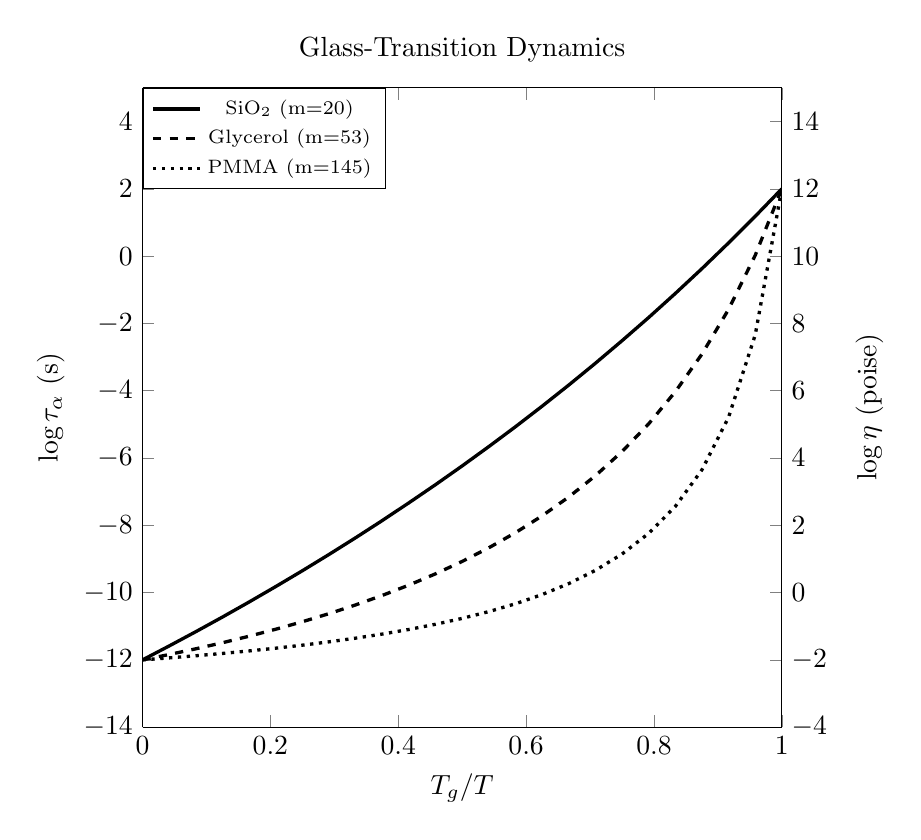
\begin{tikzpicture}[>=latex]
		\begin{axis}[
			width=0.8\textwidth,
			height=0.8\textwidth,
			xmin=0,xmax=1,
			ymin=-4,ymax=15,
			xtick=\empty,
			domain=0:15,
			axis y line*=right,
			axis x line*=none,
			y label style={at={(axis description cs:1.1,.5)},anchor=north},
			ylabel={$\log\eta$ (poise)},
			]
		\end{axis}
		
		\begin{axis}[
			legend style={at={(0,1)},anchor=north west},
			title={Glass-Transition Dynamics},
			width=.8\textwidth,
			height=.8\textwidth,
			axis y line*=left,
			xmin=0,xmax=1,
			ymin=-14,ymax=5,
			ylabel={$\log\tau_\alpha$ (s)},
			xlabel={$T_g/T$},
			]
			\addplot expression[domain=0:1,black, very thick, solid, mark=none]{
				-44.6666666667 - 108.8888888889/(x - 3.3333333333)
			}; 
			\addlegendentry{{\scriptsize SiO\textsubscript{2} (m=20)}}
			
			\addplot expression[domain=0:1,black, very thick, dashed,mark=none]{
				-17.0256410256 - 6.8297172913/(x - 1.3589743590)
			}; 
			\addlegendentry{{\scriptsize Glycerol (m=53)}}
			
			\addplot expression[domain=0:1,black, very thick, dotted,mark=none]{
				-13.4961832061 - 1.6560806480/(x - 1.1068702290)
			};
			\addlegendentry{{\scriptsize PMMA (m=145)}}
		\end{axis}
	\end{tikzpicture}
	
	\caption{Representative Angell plots illustrating the fragility of three glass-forming systems. These curves are idealized constructions chosen to reproduce the accepted ambient-pressure fragility values and are not intended to represent experimental data. Both the glass-transition and high-temperature limits are imposed to define a common dynamic range. In this representation, each system is scaled by its respective glass transition temperature $T_g$, allowing direct comparison on a common framework. Strong (Arrhenius) liquids display approximately linear behavior, whereas fragile liquids exhibit pronounced super-Arrhenius curvature as $T_g$ is approached.}
	\label{figure:AngellPlot}
\end{figure}

\noindent The Angell plot, shown in \fig\nolinebreak\ref{figure:AngellPlot}, provides a compact and intuitive representation of glass-forming dynamics. In this representation, the logarithm of either the viscosity, $\eta$, or the structural relaxation time, $\tau_\alpha$, is plotted as a function of inverse temperature normalized by the glass-transition temperature, $T_g/T$. These quantities are related through the Maxwell relation,

\begin{equation}
	\eta = G_\infty \tau_\alpha,
\end{equation}

\noindent where $G_\infty$ is the high-frequency (instantaneous) shear modulus. This relation allows either viscosity or structural relaxation time to serve as a measure of the underlying dynamics.

The horizontal axis of a classic Angell plot progresses from high temperature on the left to the glass transition at $T_g/T = 1$ on the right. This representation highlights the enormous dynamic range spanned by glass-forming liquids, with viscosity or relaxation time changing by many orders of magnitude as the system is supercooled toward $T_g$. Because each system is normalized by its own glass-transition temperature, Angell plots enable direct comparison across materials with widely differing intermolecular interactions and absolute timescales.

If one defines the high-temperature asymptotic limit as the regime in which the average thermal energy of any given molecule greatly exceeds the characteristic intermolecular interaction energies, then intermolecular constraints cease to dominate the structural dynamics of the liquid. In this regime, the system approaches behavior characteristic of weakly interacting particles, and relaxation is governed primarily by intrinsic molecular parameters rather than cooperative rearrangements. Although the liquid phase itself will ultimately lose thermodynamic stability at sufficiently high temperature, within the accessible liquid domain the relaxation dynamics progressively lose sensitivity to collective structural constraints.

As intermolecular barriers become energetically insignificant relative to $k_{B}T$, the system samples the potential energy landscape with minimal constraint. Structural relaxation is therefore controlled primarily by internal molecular properties such as moments of inertia and local conformational flexibility. Most small organic molecules span only a few angstroms, and even larger macromolecules exhibit local flexibility on comparable length scales. Consequently, the characteristic microscopic times associated with molecular motion tend to fall within similar ranges across many liquids. It is therefore not surprising that, under a given isobaric condition, liquids exhibit high-temperature asymptotic relaxation times $\tau_{\alpha}$ confined to a relatively narrow window, typically from hundreds of femtoseconds to a few picoseconds.

\fig\nolinebreak\ref{figure:AngellPlot} shows the Angell plot for three distinct glass-forming systems. Molten silicon dioxide serves as a classic example of an Arrhenius, or what Angell termed a ``strong'' liquid. Glycerol provides an example of a liquid intermediate in fragility, while the polymer PMMA exhibits highly super-Arrhenius behavior characteristic of a fragile system. Although these materials differ significantly in their intermolecular bonding---from network-forming covalent structures in \ce{SiO2}, to hydrogen bonding in glycerol, to van der Waals-dominated interactions in simple molecular liquids such as cumene, and to polymeric systems such as PMMA---fragility itself does not necessarily reflect bond strength. Rather, it characterizes how strongly the relaxation dynamics depend on temperature as the glass transition is approached.

Common network-forming liquids, such as silicates, exhibit nearly linear behavior on an Angell plot and are referred to as ``strong'' glass formers. This corresponds to an approximately Arrhenius temperature dependence of the viscosity or structural relaxation time. In contrast, many glass-forming liquids exhibit pronounced curvature in this representation, reflecting strong deviations from Arrhenius behavior. These systems are referred to as ``fragile'' glass formers.

Fragility therefore provides a quantitative measure of the degree to which a liquid’s dynamics deviate from Arrhenius behavior as the glass transition is approached. The Angell plot provides a compact means to compare the dynamics of different glass-forming systems on a single graph while simultaneously visualizing their fragilities. As defined in \eqn\nolinebreak\ref{eqn:fragility}, fragility is geometrically represented as the slope of the Angell plot at $T_g/T = 1$, \ie, as the system approaches the glass transition from the liquid state. Thus, the relative fragilities of different liquids---or of a single liquid under varying pressure---can be determined at a glance.

\begin{equation}
	m=\left ( \frac{\partial \log_{10}\eta}{\partial \left ( T_g/T \right )} \right )_{T=T_g}
	\label{eqn:fragility}
\end{equation}

\noindent This definition is inherently isobaric, as it is constructed from temperature-dependent measurements performed at fixed pressure. While Angell’s original definition emphasizes temperature-dependent behavior, comparable dynamical changes occur under compression, setting the stage for the pressure-dependent investigations presented in this work.

Because the horizontal axis of a proper Angell plot progresses from zero to one as $T_g/T$ increases, and many liquids exhibit a comparable high-temperature asymptotic viscosity on the order of $10^{-3}$--$10^{-4}$~p, the minimum fragility attainable under the conventional definition corresponds to the slope of a straight line connecting this asymptotic viscosity to that at which the glass transition is defined to occur. Taking $\eta_g \equiv 10^{13}$~p, a nearly Arrhenius liquid therefore exhibits a fragility on the order of $m \approx 16$.

Although the conventional fragility is defined as the slope of the Angell plot at $T_g$, the choice of $T_g$ itself---fixed by selecting a particular dynamical value---implicitly embeds the dynamic range into the definition. As a result, even a perfectly Arrhenius liquid does not assume a value of unity. It is therefore more natural to rescale the ordinate of the Angell representation and redefine fragility accordingly, such that an Arrhenius liquid serves as the reference case with scaled fragility equal to one.

\begin{equation}
	m^*=\frac{1}{\log_{10}\left( \frac{\eta_g}{ \eta_\infty}\right )} \left ( \frac{\partial \log_{10}\left( \frac{\eta}{ \eta_\infty}\right )}{\partial \left ( T_g/T \right )} \right )_{T=T_g}
	\label{eqn:scaledfragility}
\end{equation}

In practice, this redefinition merely rescales the classic Angell fragility by a constant normalization factor. It introduces no additional complexity into the analysis, yet it enforces well-defined high- and low-temperature limits in the Angell representation and removes ambiguity in interpretation: a purely Arrhenius system exhibits a scaled fragility of precisely $m^{\ast}=1$. By embedding the dynamic range explicitly within the definition, the scaled fragility also facilitates consistent comparison between viscosity data and structural relaxation measurements.

\begin{figure}[!htbp]
	\centering
	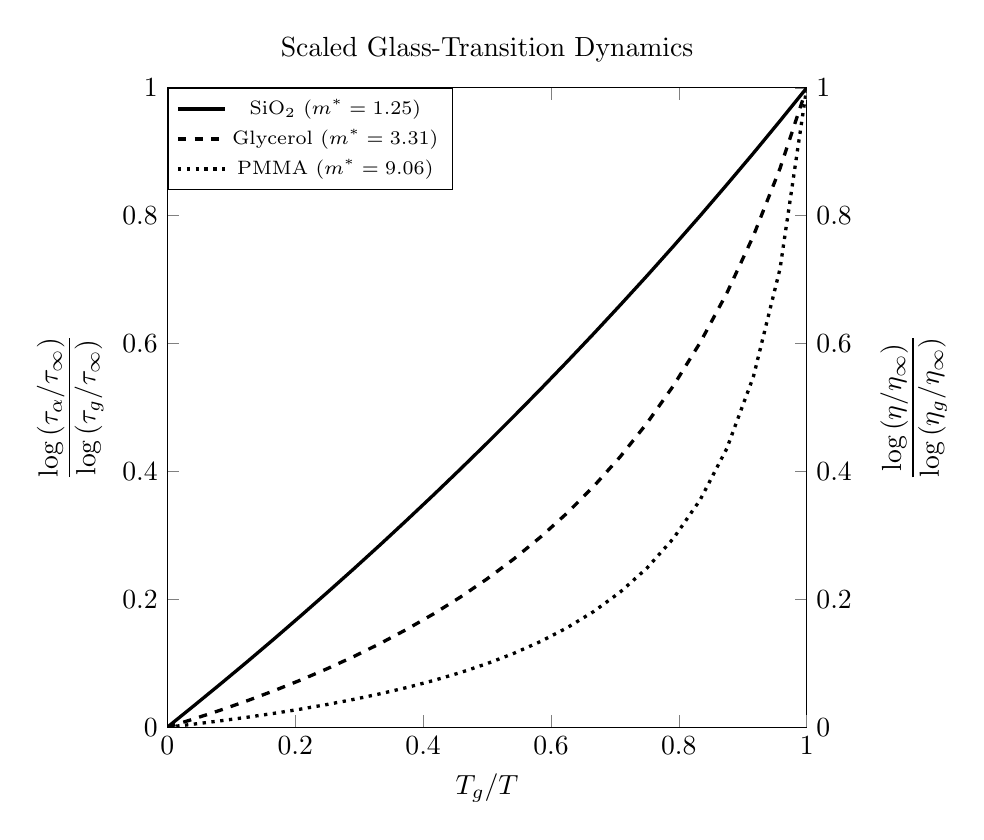
\begin{tikzpicture}[>=latex]
		\begin{axis}[
			width=0.8\textwidth,
			height=0.8\textwidth,
			xmin=0,xmax=1,
			ymin=0,ymax=1,
			xtick=\empty,
			axis y line*=right,
			axis x line*=none,
			y label style={at={(axis description cs:1.1,.5)},anchor=north},
			ylabel={$\displaystyle \frac{\log\left(\eta/\eta_\infty\right)}{\log\left(\eta_g/\eta_\infty\right)}$},
			]
		\end{axis}
		
		\begin{axis}[
			legend style={at={(0,1)},anchor=north west},
			title={Scaled Glass-Transition Dynamics},
			width=.8\textwidth,
			height=.8\textwidth,
			axis y line*=left,
			xmin=0,xmax=1,
			ymin=0,ymax=1,
			ylabel={$\displaystyle \frac{\log\left(\tau_\alpha/\tau_\infty\right)}{\log\left(\tau_g/\tau_\infty\right)}$},
			xlabel={$T_g/T$},
			]
			\addplot expression[domain=0:1,black, very thick, solid, mark=none]{
				log10(10^(-78-320/(x-5))/10^(-14))/16
			};
			\addlegendentry{{\scriptsize SiO\textsubscript{2} ($m^*=1.25$)}}
			
			\addplot expression[domain=0:1,black, very thick, dashed, mark=none]{
				log10(10^(-20.9189-9.91088/(x-1.43243))/10^(-14))/16
			};
			\addlegendentry{{\scriptsize Glycerol ($m^*=3.31$)}}
			
			\addplot expression[domain=0:1,black, very thick, dotted, mark=none]{
				log10(10^(-15.9845-2.23064/(x-1.12403))/10^(-14))/16
			};
			\addlegendentry{{\scriptsize PMMA ($m^*=9.06$)}}
		\end{axis}
	\end{tikzpicture}
	
	\caption{Scaled Angell plots for the same three liquids shown in \fig\nolinebreak\ref{figure:AngellPlot}, constrained at both the glass transition and in the high-temperature limit. In this representation, the dynamic range is normalized such that a purely Arrhenius liquid exhibits a scaled fragility of $m^{\ast}=1$.}
	\label{figure:ScaledAngellPlot}
\end{figure}

The scaled Angell plot shown in \fig\nolinebreak\ref{figure:ScaledAngellPlot} retains the same qualitative behavior as \fig\nolinebreak\ref{figure:AngellPlot}. In the classic Angell representation, the high-temperature asymptotic viscosities or relaxation times are not constrained to coincide, so the curves remain vertically offset at low $T_g/T$. By contrast, the scaled representation normalizes by the total dynamic range between the high-temperature asymptote and the glass-transition point, allowing direct comparison across systems with differing intrinsic viscosity spans. In this representation, both viscosity and structural relaxation data share a common dimensionless scale.

Importantly, many glass-forming liquids exhibit a similar limiting behavior at high temperatures, where relaxation dynamics approach a common Arrhenius-like regime. The scaled Angell representation leverages this convergence by explicitly normalizing both the high-temperature limit and the glass-transition point. In doing so, it provides a more rigorous and universal definition of fragility, wherein the minimum possible scaled fragility is, by construction, $m^* = 1$.

This work is certainly not the first to suggest an adaptation to fragility. Various alternative definitions and reinterpretations appear throughout the literature. However, the scaled fragility adopted here is particularly useful because it preserves the intuitive geometrical meaning of the Angell slope while removing the arbitrary offset imposed by the conventional dynamic range. This normalization removes ambiguity associated with differing experimental probes and absolute timescales, allowing deviations from Arrhenius behavior to be compared on an equal footing across materials.

One of the central aims of this work is to extend these concepts beyond ambient conditions and investigate how fragility evolves under compression. By incorporating pressure as an additional thermodynamic variable, it becomes possible to explore fragility not as a single scalar quantity, but as a property defined over a continuous thermodynamic surface.

\subsection{Arrhenius Systems} \label{sec:Arrhenius}

Arrhenius, or ``strong,'' glass-forming liquids are those whose primary structural relaxation exhibits an approximately temperature-independent activation energy as the glass transition is approached. In such systems, structural rearrangement occurs through thermally activated processes, with the probability of overcoming an energy barrier $\Delta E$ governed by Boltzmann statistics. Consequently, the relaxation time and viscosity follow an exponential dependence on inverse temperature,

\begin{equation}
	\tau_\alpha=\tau_\infty  \exp\left [ \frac{\Delta E}{k_{B}T} \right ]
	\label{eqn:arrhenius}
\end{equation}

\noindent where $\tau_\infty$ represents the high-temperature asymptotic relaxation time corresponding to the limit in which intermolecular constraints no longer significantly impede molecular motion.

A classic example is silicon dioxide (SiO\textsubscript{2}), which exhibits nearly linear behavior on an Angell plot, consistent with Arrhenius dynamics. Such systems approach the minimum fragility limit, typically $m \approx 15$--$16$ in the conventional definition, reflecting the fixed dynamic range embedded in the Angell representation. 

\subsection{Non-Arrhenius Systems}

Most glass-forming liquids do not exhibit purely Arrhenius behavior. Even systems typically classified as ``strong,'' such as SiO\textsubscript{2}, display some degree of curvature on an Angell plot, indicating deviations from a single, temperature-independent activation energy. In realistic systems, the presence of multiple relaxation pathways lead to a distribution of energy barriers, giving rise to non-Arrhenius dynamics.

Glass-forming liquids that exhibit pronounced deviations from Arrhenius behavior are referred to as ``fragile'' glass formers. In these systems, the effective activation energy governing structural relaxation becomes temperature dependent. At high temperature, the apparent activation energy is relatively small, but as the glass transition is approached, the effective barrier increases, leading to strongly super-Arrhenius behavior. A PMMA melt is a classic example of a fragile glass-forming liquid, while glycerol is typically considered to exhibit intermediate fragility.

The terminology ``strong'' and ``fragile,'' introduced by Angell, refers specifically to the temperature dependence of the relaxation dynamics and not to mechanical strength in the conventional sense. ``Strong'' liquids exhibit nearly Arrhenius behavior, indicating a relatively weak temperature dependence of the activation barrier, whereas ``fragile'' liquids display pronounced super-Arrhenius behavior, reflecting a rapidly increasing effective barrier as the glass transition is approached. These terms are therefore best understood as describing dynamical sensitivity to temperature rather than any intrinsic mechanical property of the material.

Fragility in such systems may also be pressure-dependent. Glycerol provides a notable example, as its fragility increases with increasing pressure, an effect attributed to the suppression of hydrogen bonding. This pressure dependence will be explored in detail in \chap\nolinebreak\ref{chap:Glycerol}.

The temperature dependence of non-Arrhenius dynamics is commonly described using the Vogel--Tammann--Fulcher (VTF) equation, first proposed by Tammann and Hesse in 1926, to describe the temperature dependence of viscosity in polar liquids \cite{Tammann}.  The modern form of this equation, most prevalent in the literature, is given by

\begin{equation}
	\centering
	\tau_\alpha=\tau_\infty  \exp\left [ \frac{DT_0}{T-T_0} \right ]
	\label{eqn:VTFintro}
\end{equation}

\noindent where $T_0$ is the extrapolated temperature at which the relaxation time diverges, often referred to as the zero-mobility temperature, and $D$ is a material-dependent parameter related to fragility. This form captures the rapid growth of relaxation times as the system approaches the glass transition from the liquid state.

\section{Dielectric Fluctuations and Light Scattering}
\label{sec:TheScatteredField}

Any time light travels through a transparent medium, electromagnetic fields couple with charges within the medium, inducing electronic moments. This interaction can be quite complicated, resulting in a scattered field that requires a multipole expansion to describe properly. However, in the limit where the wavelength of the incident field is large compared to the characteristic microscopic length scales within the medium, the electric dipole term generally dominates and the induced polarization may be treated in the quasi-static (long-wavelength) limit, where spatial variations of the field across a scattering region are negligible \cite[p.~572]{Jackson}. 

The general form of the scattered field, though technically a quantum effect, can be derived via classical electrodynamic theory and is well described in general terms by both Jackson and Landau–Lifshitz, while Berne and Pecora offer a more practical rendition of Landau’s derivation specifically in the context of dynamic light scattering\nolinebreak \cite{Landau,Jackson,Berne}. In all cases, an incident monochromatic plane wave is assumed to propagate through a scattering medium as depicted in \fig \nolinebreak \ref{figure:planescatter}.

An incident monochromatic plane wave, indicated by the vertical blue lines, propagates in the $+\hat{z}$ direction with wavevector
\begin{equation}
\vec{k}_{in} = \frac{2 n \pi}{\lambda_{in}},
\end{equation}
where $\lambda_{in}$ is the incident wavelength in vacuum and $n$ is the refractive index of the medium. Light scattered by the medium is collected at a scattering angle $\theta_S$ relative to the incident direction, as indicated by the dashed arrows, with outgoing wavevector

\begin{equation}
\vec{k}_{out} = \frac{2 n \pi}{\lambda_{out}}.
\end{equation}

Typical laser wavelengths used in light-scattering experiments are on the order of $\lambda_{in} \approx 500~\text{nm}$, corresponding to optical frequencies near $6\times10^{14}~\text{Hz}$. For a representative refractive index of $n \approx 1.4$, the magnitude of the incident wavevector is therefore
\begin{equation}
k_{in} \approx \frac{2(1.4)\pi}{500\times10^{-9}\,\text{m}} \approx 1.8\times10^{7}~\text{m}^{-1}.
\end{equation}

In inelastic Brillouin light scattering, the scattered light typically differs in frequency from the incident light by at most a few gigahertz, while in quasi-elastic photon correlation spectroscopy (PCS), the frequency shifts range from sub-hertz to megahertz. In either case, these shifts are negligible compared to the optical carrier frequency. It is therefore an excellent approximation to assume $\lambda_{out} \approx \lambda_{in}$, so that $|\vec{k}_{out}| \approx |\vec{k}_{in}| \equiv k$. Under this assumption, the scattering vector
\begin{equation}
\vec{q} = \vec{k}_{out} - \vec{k}_{in}
\end{equation}
\noindent has magnitude, via the law of cosines,
\begin{equation}
q = 2k \sin\left(\frac{\theta_S}{2}\right).
\end{equation}
\noindent This long-wavelength approximation, in which the incoming and outgoing wavelengths are effectively identical, constitutes one of the primary assumptions underlying the analysis that follows.

For typical scattering angles employed in Brillouin light-scattering experiments, $q$ is on the same order as $k_{in}$, and the frequencies of the Stokes and anti-Stokes Brillouin shifts are determined by the acoustic velocity $v$ of the medium according to
\begin{equation}
\nu = \frac{q v}{2\pi}.
\end{equation}

In PCS experiments on simple fluids, the relevant density fluctuations occur over spatial scales that are small compared to the wavelength, provided the system is not near a critical point where macroscopic critical fluctuations would dominate \cite{Stanley1971}. Although dynamic heterogeneities grow as the glass transition is approached, their characteristic length scales remain on the order of only a few molecular diameters (i.e., nanometers), far below optical wavelengths in typical glass-forming liquids~\cite{BerthierBiroli2011,Ediger2000}. In this limit, the electromagnetic field is effectively uniform across each microscopic scattering region, and all molecules within that region experience essentially the same local electric field. The total scattering volume in an experiment then consists of many such statistically independent regions, and the scattered light collected represents the coherent superposition of the fields radiated by each region. This physical picture of light scattering from thermodynamic density fluctuations was first articulated by Einstein in his early treatment of critical opalescence \cite{Einstein1910}.


\begin{figure}[!htbp]
	\centering
	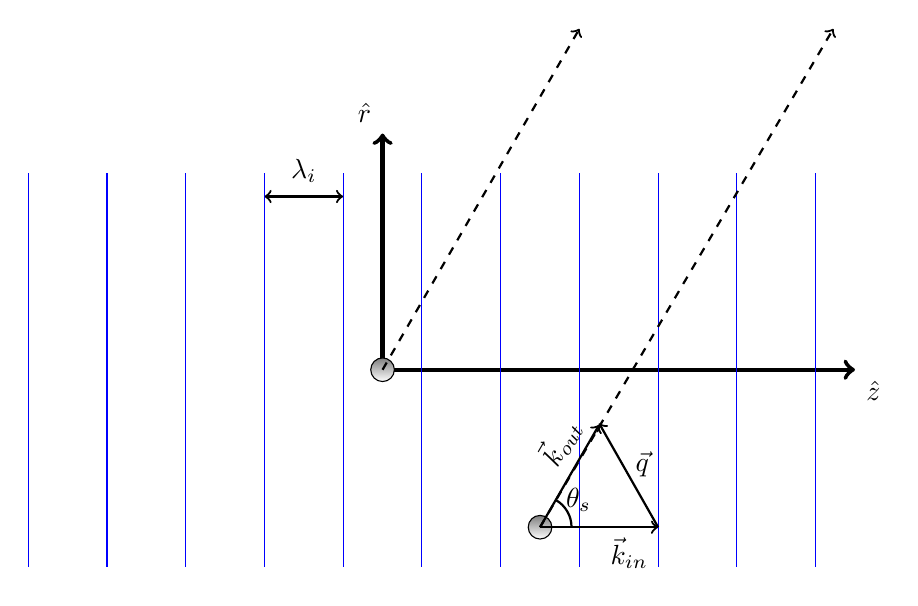
\begin{tikzpicture}
		%Z-Axis
		\draw[ultra thick,->] (0,0) -- (6,0) node[anchor=north west] {$\hat{z}$};
		\draw[ultra thick,->] (0,0) -- (0,3) node[anchor=south east] {$\hat{r}$};
		
		% Wavelength indicator (top left)
		\draw[<->, thick] (-1.5,2.2) -- (-0.5,2.2);
		\node[anchor=south] at (-1.0,2.25) {$\lambda_i$};
		
		
		\foreach \x in {-4,-3,-2,-1,0,1,2,3,4,5,6}
		\draw[thin, blue] (\x-.5,-2.5) -- (\x-.5,2.5);
		\draw[shade] (2,-2) circle (0.15cm);
		\draw[shade] (0,0) circle (0.15cm);
		
		%K Vectors
		\draw[thick,->]  (2,-2) -- (3.5,-2)  node[anchor=north east] {$\vec{k}_{in}$};
		\draw[thick,->] (2,-2) -- (2.75,-0.700961894) node[anchor=south east,rotate=60] {$\vec{k}_{out}$};
		\draw[thick,<-] (2.75,-0.68)--(3.5,-2); 
		\node[] at (3.3,-1.2) {$\vec{q}$};
		%arc for scatter vector
		\draw[thick] (2.4,-2) arc (0:60:.4) node[anchor=west] {$\theta_{s}$};
		
		%dotted rays
		\draw[dashed,black, thick,->] (0,0) -- (5*.5,5*.866025);
		\draw[dashed,black, thick,->] (2,-2) -- (5*1.145,5*.866025);
	\end{tikzpicture}
	\caption{Vertical lines represent a plane wave propagating in the $\hat{z}$ direction into a region of dispersed scattering bodies. The time-dependent dipole moments induced in each molecule or particle act as independent sources of a scattered field. Here we assume a diffuse scattering medium such that secondary scattering events contribute negligibly to the net scattered field\nolinebreak \cite{Berne}.}\label{figure:planescatter}
\end{figure}

For scattering to serve as an effective structural probe, the medium must be optically thin such that higher-order multiple scattering contributions are negligible. In this dilute (or optically thin) limit, the detected scattered field is linear in the dielectric fluctuation $\delta\epsilon$, and light collected at an angle $\theta_s$ may be associated with a well-defined scattering vector $\vec{q} = \vec{k}_{out} - \vec{k}_{in}$. Because the incident wavevector $\vec{k}_{in}$ is known and the collection geometry fixes $\vec{k}_{out}$, the scattering vector $\vec{q}$ is likewise well defined and will play a central role in the analysis that follows.

To build intuition for the light-scattering process, one may first consider a system in which the local number density of scatterers fluctuates in time due to thermal motion. In a dilute suspension of particles, such fluctuations arise from Brownian motion. In condensed phases, including simple liquids, analogous fluctuations occur as molecules move and create short-lived variations in local density within the bulk.

Thus, to describe how light is scattered from a bulk medium, one must recognize that the dielectric permittivity of any real material fluctuates—both temporally and spatially—due to the random thermal motions of the constituent particles or molecules, as well as any structural inhomogeneities. This can be modeled as a static ``average'' permittivity around which local fluctuations occur as follows:

\begin{equation}
	\centering
	\epsilon\left(\vec{r},t\right)=\epsilon I + \delta\epsilon\left(\vec{r},t\right).
	\label{eqn:dielectricflux}
\end{equation}

Here $\epsilon$ is the scalar dielectric permittivity of the medium, and $\delta\epsilon$ describes deviations from this constant, which in general depend on both space and time and may include off-diagonal elements, providing a completely general description of local permittivity in any transparent medium.  

From this point we derive the wave equation for the scattered field to understand what gives rise to it. Landau–Lifshitz and Jackson provide excellent classical derivations, while Berne and Pecora give a simplified treatment specific to light scattering\nolinebreak \cite{Landau,Jackson,Berne}. As illustrated in \fig \nolinebreak \ref{figure:planescatter}, if a plane wave traveling through a medium is to produce a scattered field, the resulting field in the medium is the superposition of the incident and scattered fields:

\begin{eqnarray}
	&E=E_i+E_s, \label{eqn:fieldsplusscatter1} \\ 
	&D=D_i+D_s, \label{eqn:fieldsplusscatter2} \\ 
	&H=H_i+H_s. \label{eqn:fieldsplusscatter3}
\end{eqnarray}

Whatever form the scattering fields assume, they must satisfy Maxwell’s equations for fields within a medium, where we assume nonmagnetic materials appropriate for this dissertation.
\begin{eqnarray}
	&\nabla \times E_s=-\frac{1}{c}\frac{\partial H_s}{\partial t}, \label{eqn:Maxwell1}\\
	&\nabla \times H_s=\frac{1}{c}\frac{\partial D_s}{\partial t}, \label{eqn:Maxwell2}\\
	&\nabla \cdot  H_s=0, \label{eqn:Maxwell3}\\
	&\nabla \cdot  D_s=0. \label{eqn:Maxwell4}
\end{eqnarray}

From \eqn\nolinebreak \ref{eqn:Maxwell1} and \eqn\nolinebreak \ref{eqn:Maxwell2} one obtains:
\begin{equation}
	\nabla \times \nabla \times E_s=-\frac{1}{c^2}\frac{\partial^2 D_s}{\partial t^2}.
	\label{eqn:MaxwellEresult}
\end{equation}

The net instantaneous displacement vector from \eqn\nolinebreak \ref{eqn:fieldsplusscatter2} is related to the electric field vector from \eqn \ref{eqn:fieldsplusscatter1} by the dielectric tensor from \eqn\nolinebreak \ref{eqn:dielectricflux}:
\begin{equation}
	D_i+D_s=\left(\epsilon I + \delta\epsilon\left(\vec{r},t\right)\right)\cdot \left(E_i+E_s \right ).
\end{equation}

Solving for the scattering field $E_s$ and neglecting the $\delta\epsilon\cdot E_s$ term that would give rise to secondary scattering of much smaller magnitude:
\begin{equation}
	E_s=\frac{1}{\epsilon}D_s-\frac{1}{\epsilon}\left(\delta \epsilon\cdot E_i\right).
\end{equation}

This scattering field must satisfy \eqn\nolinebreak \ref{eqn:MaxwellEresult}:
\begin{equation}
	\nabla \times \nabla \times D_s-\nabla \times \nabla \times \left(\delta \epsilon\cdot E_i\right)=-\frac{\epsilon}{c^2}\frac{\partial^2 D_s}{\partial t^2}.
\end{equation}

Utilizing Lagrange’s cross-product identity and \eqn \ref{eqn:Maxwell4}, this simplifies to:
\begin{equation}
	\nabla^2D_s-\frac{\epsilon}{c^2}\frac{\partial^2 D_s}{\partial t^2}=-\nabla\times\nabla\times\left(\delta\epsilon\cdot E_i\right).
	\label{eqn:waveequation}
\end{equation}

\eqn\nolinebreak \ref{eqn:waveequation} is a wave equation for the scattering displacement vector $D_s$ with a source term proportional to $\delta\epsilon\cdot E_i$. This derivation assumes only that fields satisfy Maxwell’s equations and that the dielectric permittivity is described by the tensor in \eqn\nolinebreak \ref{eqn:dielectricflux}.  
 
 \section{Spectrum of a Simple Fluid} \label{sec:SpectrumOfSimpleFluid}
 Until this point, the scattering field has been discussed in very general terms.  Moving forward the discussion will be focused on the application at hand\textemdash light scattering as a probe of molecular dynamics.  As such, the incident field, $E_i$, will be assumed to be a monochromatic constant intensity laser light source passed through a transparent fluid from which scattered light will be collected along a specific scattering vector as shown in \fig \nolinebreak \ref{figure:scatterSetup}.
 \begin{figure}[!htbp]
 	\centering
	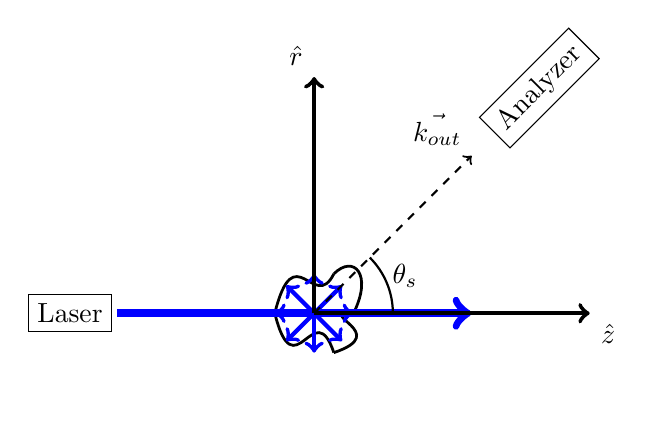
\begin{tikzpicture}
 
 		%Scattering Volume
 		\draw[line width=1pt] (0,0) .. controls (.25,1) and (.5,0) .. (.75,.5);
 		\draw[line width=1pt] (.75,.5) .. controls (1,.75) and (1.25,.5) .. (1,0);
 		\draw[line width=1pt] (1,0) .. controls(.5,0) and (1.5,-.25) .. (.75,-.5);
 		\draw[line width=1pt] (.75,-.5) .. controls (.5,.25) and (.25,-1) .. (0,0);
 
 		%Incident and Scattered Field Vectors
		\draw [->,line width=3pt,blue] (-2,0) -- (2.5,0);
 		\draw [->,line width=1.5pt,blue] (.5,0) -- (.5,.5);
 		\draw [->,line width=1.5pt,blue] (.5,0) -- (.146447,.5*.707107);
 		\draw [->,line width=1.5pt,blue] (.5,0) -- (.853553,.5*.707107);
 		\draw [->,line width=1.5pt,blue] (.5,0) -- (1,0);
 		\draw [->,line width=1.5pt,blue] (.5,0) -- (0,0);
 		\draw [->,line width=1.5pt,blue] (.5,0) -- (.5,-.5);
 		\draw [->,line width=1.5pt,blue] (.5,0) -- (.146447,-.5*.707107);
 		\draw [->,line width=1.5pt,blue] (.5,0) -- (.853553,-.5*.707107);
 
 		%Z-Axis
 		\draw[ultra thick,->] (.5,0) -- (4,0) node[anchor=north west] {$\hat{z}$};
 		\draw[ultra thick,->] (.5,0) -- (.5,3) node[anchor=south east] {$\hat{r}$};
 
 		%dashed Scattering Vector
 		\draw[thick, dashed,->] (.5,0) -- (2.5,2) node[anchor=south east] {$\vec{k_{out}}$};
 
 		%arc for scatter vector
 		\draw[thick] (1.5,0) arc (0:45:1);
 		\node[] at (1.654849,.478354) {$\theta_{s}$};
 
 		\node[draw, rotate=45] at (3.360077,2.860077) {Analyzer};
 		\node[draw] at (-2.6,0) {Laser};
 
 	\end{tikzpicture}
 	\caption{Generalized light scattering geometry}
 	\label{figure:scatterSetup}
 \end{figure}
 
It is important to quantify the length scales relevant to the scattering volume in order to justify the continuum treatment used in the derivation of \eqn\nolinebreak \ref{eqn:waveequation}. For a typical focused laser beam used in light scattering experiments, the beam waist may be on the order of $w_0 \sim 50$--$100~\mu$m, while the effective scattering length defined by the collection optics is on the order of $L \sim 1$--$5~\text{mm}$. This corresponds to a scattering volume of approximately
\begin{equation}
	V \sim \pi w_0^2 L \approx 10\text{--}150~\text{nL}.
\end{equation}

\noindent For a typical molecular liquid with number density in the ballpark of $n \sim 10^{13}~\text{nL}^{-1}$, the scattering volume lies well within the continuum limit.

This should be contrasted with the characteristic intermolecular spacing, $a \sim 0.3$--$0.5~\text{nm}$, which is many orders of magnitude smaller than both the optical wavelength ($\lambda \sim 500~\text{nm}$) and the spatial extent of the scattering volume. As a result, the measured scattering signal arises from the collective response of an enormous number of molecules, and fluctuations in the dielectric susceptibility emerge from statistically averaged molecular motions that are effectively uncorrelated on optical length scales. Within any fluid above absolute zero there will be local regions where bulk thermodynamic properties such as entropy, temperature, or pressure will fluctuate about the average value.  It is these fluctuations, as alluded to previously, that give rise to the scattering field.  Thus, it is reasonable to invoke hydrodynamic and thermodynamic theory to arrive at a model for the spectrum of light scattered from a simple fluid.  Such a model was first derived by Komarov and Fisher in their 1962 publication\cite{Komarov}. In this work Komarov adapted neutron scattering models derived by Leon van Hove in 1954 to describe light scattering spectra\cite{Hove}. It should be noted that this derivation is also provided in excellent detail by Berne and Pecora \nolinebreak \cite{Berne}.  The resulting spectrum of this scattered light was shown by Komarov to be proportional to the spatial and temporal Fourier transform of the generalized pair correlation function. While \sect \ref{sec:sctructualdesc} introduced the static radial distribution function describing equilibrium structure, it is necessary here to consider its dynamical extension. 

Following the work of van Hove, the static pair correlation function is generalized to the time-dependent van Hove correlation function $G(\vec{r},t)$, which describes the probability of finding a particle at position $\vec{r}$ at time $t$ given that a particle was located at the origin at time $t=0$. The dynamic structure factor $S(\vec{q},\omega)$ is then obtained as the spatial and temporal Fourier transform of $G(\vec{r},t)$. The scattered intensity may therefore be written as
\begin{equation}
	I^\prime\left(\vec{r},\omega\right)
	=
	I_0 N \omega^4 \sin^2{\gamma}\,
	S\left(\vec{q},\omega\right),
\end{equation}
\noindent where $I_0$ is the incident intensity, $N$ is the number of scatterers within the scattering volume, $\omega$ is the angular frequency of the incident field, and $\gamma$ is the angle between the induced dipole moment and the observation direction, giving rise to the characteristic dipole radiation pattern. Here $\vec{q} = \vec{k}_s - \vec{k}_i$ is the scattering wavevector.

This result is closely related to that for Rayleigh scattering from a diffuse gas, with the addition of the structure factor, $S\left(\vec{q},\omega \right)$, which contains information about the molecular dynamics of the system. Mountain later extended the results of Komarov and Fisher and through application of the linearized hydrodynamic equations, which include the continuity equation, Navier--Stokes, and energy-transport equations, derived a model for the frequency-dependent structure factor of a classical fluid comprised of spherically symmetric molecules as follows:
\begin{equation}
\centering
S\left(q,\omega \right )=\frac{c_p-c_v}{c_p}\frac{2\lambda q^2/\rho_0c_p}{\left(\lambda q^2/\rho_0c_p \right )^2+\omega^2}+\frac{c_v}{c_p}\left [ \frac{\Gamma q^2}{\left(\Gamma q^2 \right )^2+\left(\omega+C_0 q \right )^2}+ \frac{\Gamma q^2}{\left(\Gamma q^2 \right )^2+\left(\omega-C_0 q \right )^2}\right ].\label{eqn:simpleFluid}
\end{equation}
Here $\rho_0$, $c_p$, $c_v$, $C_0$, and $\lambda$ are the equilibrium density, specific heat at constant pressure, specific heat at constant volume, low frequency limit of the sound velocity, and the thermal conductivity respectively.\cite{Mountain2}  The first, left-most term of \eqn\nolinebreak \ref{eqn:simpleFluid} represents the broadened central peak of light scattering from entropy fluctuations which occur at constant pressure.  In a simple fluid, as there are no internal degrees of freedom, this takes the form of diffusion or breaking of nearest neighbor cages\textemdash \ie, structural relaxation.  The right-most term of \eqn\nolinebreak \ref{eqn:simpleFluid} represents light scattered by propagating acoustic waves.  As this is an adiabatic process, this occurs at constant entropy.  This term forms two peaks symmetrically located around the central peak with frequency shifts from $E_i$ proportionally to the speed of sound.  These are often referred to as the longitudinal acoustic modes.  This model is sufficient to describe the dynamics of a simple fluid in the sense described by Mountain: a single-component, monatomic system in which internal degrees of freedom may be neglected and the dynamics are governed entirely by density fluctuations. However, typical glass-forming systems possess additional internal and configurational degrees of freedom, giving rise to additional modes of structural relaxation beyond those captured by this description.

Many glass-forming systems are significantly more complex, exhibiting internal degrees of freedom, intermolecular hydrogen bonding, and other additional considerations.  Polymer systems can fold and flex.  Even simple molecular systems limited to van der Waals interactions, such as cumene, have rotational degrees of freedom that give rise to additional relaxation modes.  Such considerations will add to the complexity of this structure factor.  Mountain followed this previous work with a derivation of a structure factor accounting for internal degrees of freedom weakly coupled to the originally considered translational degrees of freedom via a single representative orientational relaxation time, $\tau$ as follows \cite{Mountain}: 

\begin{align}
\begin{split}
S\left(q,\omega \right )={}& \frac{c_p-c_v}{c_p}\frac{2\lambda q^2/\rho_0c_p}{\left(\lambda q^2/\rho_0c_p \right )^2+\omega^2}+\\
& \left[\frac{\left(c^2_\infty-c^2_0\right )k^2-\left(v^2/c^2_0-1 \right )\left(c^4_0/v^4\tau^2+c^2_0q^2\left(\frac{c_p-c_v}{c_p} \right ) \right )}{c^4_0/v^4\tau^2+v^2q^2}\right]\left[\frac{\frac{2c^2_0}{v^2\tau}}{\frac{c^4_0}{v^4\tau^2}+\omega^2} \right ] +\\
& \qquad \qquad \qquad \qquad \left[\frac{\left[1-\frac{c^2_0}{v^2}\left(\frac{c_p-c_v}{c_p} \right ) \right ]\left[v^2q^2+\frac{c^2_0}{v^2\tau^2} \right ]-\left(c^2_\infty-c^2_0 \right )q^2}{\frac{c^4_0}{v^4\tau^2}+\frac{v^2}{q^2}}
\right ]\times \\
& \qquad \qquad \qquad \qquad
\left[\frac{\Gamma_B}{\Gamma^2_B+\left(\omega-vq \right )^2}+\frac{\Gamma_B}{\Gamma^2_B+\left(\omega+vq \right )^2} \right ].
\end{split}\label{eqn:intdegfluid}
\end{align}
Here the longitudinal acoustic modes represented by the third term are structurally indistinguishable from the second term of \eqn\nolinebreak \ref{eqn:simpleFluid} though now the coefficient is $\tau$ dependent.  Likewise the first term, associated with translational diffusion, remains unchanged from before.  However, most notably, there now emerges a secondary central feature symmetric about the incident frequency, associated with this internal relaxation mode. Thus the orientational dynamics directly affect the structure of this central feature.  There is a vast amount of insight provided by this model.  However the primary consideration relevant to this work lies in this additional central term of \eqn\nolinebreak \ref{eqn:intdegfluid} above.  Consider the following simplified expression of this structure.
\begin{equation}
f\left(\omega \right )=\left(\frac{2\Gamma}{\Gamma^2+\omega^2} \right )\label{eqn:simplecentral}
\end{equation}
This function, as aforementioned, will be symmetric about the axis $\omega=0$ and will have a characteristic half width half maximum value of $\Gamma$ as shown in \fig \nolinebreak \ref{figure:centralstructure}.
\begin{figure}[!htbp]
	\centering
	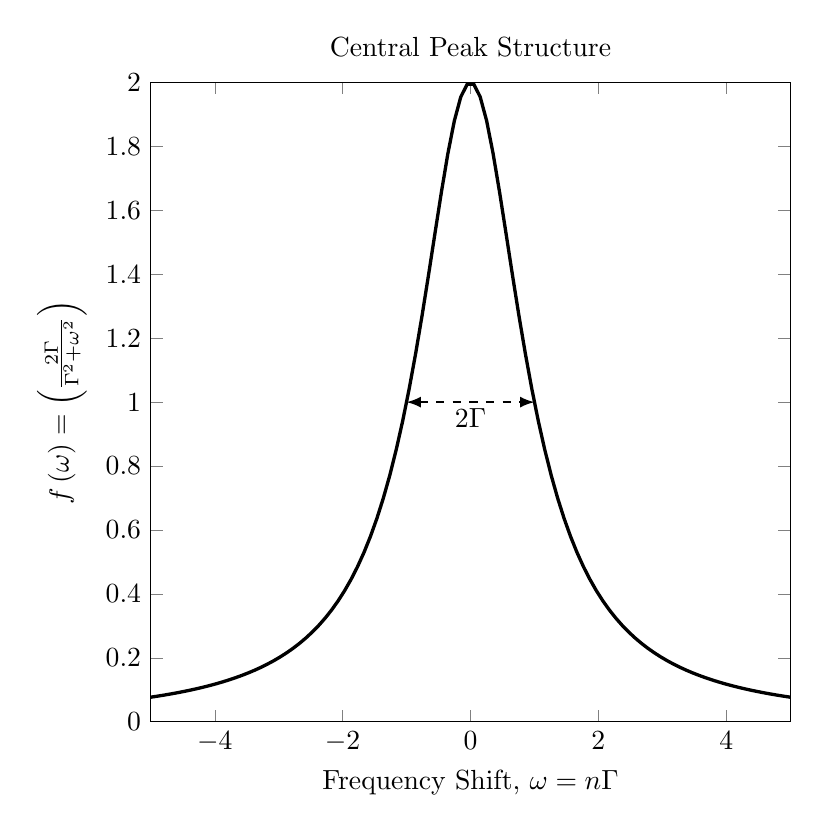
\begin{tikzpicture}[>=latex]
	
	\begin{axis}[
	samples=100,
	title={Central Peak Structure},
	width=.8\textwidth,
	height=.8\textwidth,
	xmin=-5,xmax=5,
	ymin=0,ymax=2,
	ylabel={$f\left(\omega \right )=\left(\frac{2\Gamma}{\Gamma^2+\omega^2} \right )$},
	xlabel={Frequency Shift, $\omega=n\Gamma$},
	]
	
	\addplot expression[black, very thick, solid,mark=none]{
		2/(1+x^2)}; 
	
	\draw[thick, dashed,<->] (-1,1) -- (1,1);
	\node[] at (0,.95) {$2\Gamma$};
		
	\end{axis}

	\end{tikzpicture}
	\caption{Here we have the generalized structure of the central features from \eqn\nolinebreak \ref{eqn:simpleFluid} and \nolinebreak \eqn\ref{eqn:intdegfluid}.  The x-axis here is in terms of multiples of the generalized parameter $\Gamma$ from \eqn\nolinebreak \ref{eqn:simplecentral} which also defines the half width-half maximum value for this feature.}
	\label{figure:centralstructure}
\end{figure}
Placing aside the specific values of any particular bulk thermodynamic property, both the first and second term of \eqn\nolinebreak \ref{eqn:intdegfluid} have the same basic structure in this model.  Generally speaking, the structural relaxation associated with translational and orientational diffusion can occur on vastly different timescales however both will contribute to the width of this central feature.  It bears mention that, for a simple monatomic fluid, only the translational diffusion term contributes to this central feature and $\Gamma=\frac{\lambda}{\rho_0c_p}q^2=D_Tq^2$ where $D_T$ is the thermal diffusivity and there exists a dependency on the scattering vector.  However, if the orientational diffusion contribution dominates the width of the central feature then $\Gamma=\frac{{c_0}^2}{v^2\tau}=\frac{D_\tau}{\tau}$ and there is no dependence on the scattering vector.

The work of Demoulin, Montrose, and Ostrowsky provides valuable insights and foundational support for understanding the scattering phenomena described in this chapter. Specifically, Demoulin \etal employed digital-correlation spectroscopy, analogous to photon correlation spectroscopy (PCS) utilized in this dissertation, to investigate structural relaxation in viscous liquids over time scales from $\SI{1}{\micro\second}$ to $\SI{1}{\second}$. Their work explicitly analyzed the Rayleigh scattering of light from undercooled glycerol, relating the measured correlation function to the isothermal structural relaxation dynamics of the liquid\cite{Demoulin}.

Demoulin \etal characterized three distinct regimes governing the Rayleigh line shape arising from density fluctuations: thermal diffusion dominance, structural relaxation dominance, and an intermediate regime involving contributions from both processes. Of particular interest here is what Demoulin \etal described as the "Mountain component," which appears prominently under conditions where the structural relaxation timescale is significantly slower than the phonon modes but faster than thermal diffusion processes.

This Mountain component corresponds directly to the central feature described earlier in the structural factor from \eqn\nolinebreak \ref{eqn:intdegfluid}, particularly when orientational diffusion significantly influences its width. Demoulin \etal modeled the relaxation function using a Cole-Davidson distribution—precisely the approach taken in this dissertation—to quantify the relaxation dynamics, further validating the methodology adopted here. Their analysis determined that the Cole-Davidson distribution, characterized by a width parameter, provided a robust fit for their data.

Thus, the work presented in this dissertation parallels Demoulin \etal’s in both the choice of methodology (PCS) and the theoretical framework (Cole-Davidson distribution), thereby establishing continuity and credibility in the application of these techniques to characterize structural relaxation in glass-forming liquids. Furthermore, Demoulin \etal's findings underscore the importance and practicality of employing digital autocorrelation techniques to probe relaxation phenomena, reinforcing the methodologies implemented throughout this dissertation.

\section{Mathematical Models}
\label{sec:models}

In analyzing experimental data from dynamic light scattering experiments, it becomes necessary to implement mathematical models to characterize structural relaxation processes accurately. Four commonly used models—Debye relaxation, Cole-Cole, Cole-Davidson, and Williams-Watts—will be introduced, described, and compared in this section, with emphasis on their typical usage in either the time or frequency domain, and the interrelation between domains provided by Lindsey and Patterson.

\subsection{Debye Relaxation}

The Debye relaxation model represents the simplest case, assuming a single exponential decay characterizes the relaxation process. In the time domain, this corresponds to:

\begin{equation}
	\phi(t) = e^{-t/\tau_0}.
\end{equation}

\noindent where $\tau_0$ is a single characteristic relaxation time. In the frequency domain, Debye relaxation is described by:

\begin{equation}
	\phi(\omega) = \frac{1}{1 + i\omega\tau_0}.
\end{equation}

\noindent This model assumes a uniform relaxation process without distribution of relaxation times. Although appealing for simplicity, the Debye model fails to describe the complex relaxation behaviors observed in most glass-forming liquids.

\subsection{Cole--Cole Relaxation}

Recognizing deviations from ideal Debye behavior, the Cole--Cole model introduces a phenomenological broadening of the relaxation time spectrum, characterized by an additional parameter $\alpha$:

\begin{equation}
	\phi(\omega) = \frac{1}{1+(i\omega\tau_{cc})^{1-\alpha}}, \quad 0 \le \alpha < 1.
\end{equation}

\noindent where $\tau_{cc}$ is a characteristic relaxation time and $\alpha$ describes the deviation from single-exponential (Debye) relaxation. The limiting cases are instructive. For $\alpha = 0$, the expression reduces to the Debye model, corresponding to a single relaxation time and yielding a perfect semicircle when the imaginary component of the susceptibility is plotted against the real component. In contrast, as $\alpha \rightarrow 1$, the frequency dependence is suppressed and $\phi(\omega)$ approaches a constant, reflecting the absence of a well-defined relaxation process.

For intermediate values of $\alpha$, the response cannot be described by a single relaxation time. Instead, the Cole--Cole form corresponds to a distribution of relaxation times centered around $\tau_{cc}$. This behavior is most clearly visualized in a Cole--Cole plot, where increasing $\alpha$ leads to a symmetric depression of the semicircular response, as shown in \fig\nolinebreak\ref{fig:DebyeColeCole}.

\begin{figure}[!htbp]
	\centering
	\begin{tikzpicture}
		
		\begin{groupplot}[
			group style={
				group size=2 by 1,
				horizontal sep=2.2cm
			},
			width=0.42\textwidth,
			height=0.32\textwidth,
			xmin=0, xmax=1.05,
			ymin=0, ymax=0.55,
			axis lines=left,
			axis equal image,
			xlabel={$\Re[\phi(\omega)]$},
			ylabel={$-\Im[\phi(\omega)]$},
			xtick={0,0.2,0.4,0.6,0.8,1.0},
			ytick={0,0.1,0.2,0.3,0.4,0.5},
			every axis plot/.append style={thick, black},
			domain=-3:3,
			samples=300,
			unbounded coords=jump
			]
			
			% ---------------- Debye ----------------
			\nextgroupplot[
			title={Debye ($\alpha=0$)}
			]
			
			\addplot[smooth]
			(
			{1/(1 + (10^x)^2)},
			{(10^x)/(1 + (10^x)^2)}
			);
			
			\addplot[dashed, thin] coordinates {(0,0) (0.5,0.5)};
			
			% ---------------- Cole-Cole ----------------
			\nextgroupplot[
			title={Cole--Cole ($\alpha=0.35$)}
			]
			
			\addplot[smooth]
			(
			{ (1 + (10^x)^0.65*cos(deg(0.65*pi/2))) /
				((1 + (10^x)^0.65*cos(deg(0.65*pi/2)))^2 + ((10^x)^0.65*sin(deg(0.65*pi/2)))^2) },
			{ ((10^x)^0.65*sin(deg(0.65*pi/2))) /
				((1 + (10^x)^0.65*cos(deg(0.65*pi/2)))^2 + ((10^x)^0.65*sin(deg(0.65*pi/2)))^2) }
			);
			
			\addplot[dashed, thin] coordinates {(0,0) (0.50,0.28)};
			
		\end{groupplot}
		
	\end{tikzpicture}
	\caption{Generalized representations of relaxation in a Cole--Cole plot. The case $\alpha = 0$ recovers simple Debye behavior, yielding a perfect semicircle. For $\alpha = 0.35$, the response exhibits a depressed semicircle, reflecting symmetric broadening of the distribution of relaxation times. Dashed lines are drawn from the origin to the peak of each arc, which occurs at $\omega\tau = 1$ in both cases, and emphasize the reduction in slope associated with increasing $\alpha$.}
	\label{fig:DebyeColeCole}
\end{figure}

\noindent This symmetric broadening reflects the presence of multiple relaxation pathways with comparable weights, rather than a single dominant timescale. While the Cole--Cole model captures symmetric deviations from Debye behavior, many glass-forming liquids exhibit asymmetric broadening of the relaxation spectrum. This behavior is more accurately described by the Cole--Davidson model, which will be discussed subsequently.

\subsection{Cole--Davidson Relaxation}

The Cole--Davidson model extends Debye relaxation by introducing an asymmetric broadening of the relaxation time distribution, characterized by the parameter $\beta$:

\begin{equation}
	\phi(\omega) = \frac{1}{(1 + i\omega\tau_{cd})^{\beta}}, \quad 0 < \beta \le 1.
	\label{eqn:ColeDavidson}
\end{equation}

\noindent where $\tau_{cd}$ is a characteristic relaxation time and $\beta$ describes the deviation from single-exponential (Debye) relaxation.

The limiting cases are again instructive. For $\beta = 1$, the expression reduces to the Debye model, corresponding to a single relaxation time and yielding a perfect semicircle, as in the case $\alpha = 0$ for the Cole--Cole model discussed above. As $\beta$ decreases below unity, the relaxation spectrum becomes increasingly asymmetric. In the limit $\beta \rightarrow 0$, the frequency dependence is suppressed and the response approaches a constant, analogous to the $\alpha \rightarrow 1$ limit of the Cole--Cole model.

For intermediate values of $\beta$, the response cannot be described by a single relaxation time. Instead, the Cole--Davidson form corresponds to a distribution of relaxation times with a pronounced tail toward longer relaxation times. This behavior is most clearly visualized in a Cole--Davidson plot, where decreasing $\beta$ leads to an asymmetric distortion of the semicircular response, as shown in \fig\nolinebreak\ref{fig:DebyeColeDavidson}.

\begin{figure}[!htbp]
	\centering
	\begin{tikzpicture}
		
		\begin{groupplot}[
			group style={
				group size=2 by 1,
				horizontal sep=2.2cm
			},
			width=0.42\textwidth,
			height=0.32\textwidth,
			xmin=0, xmax=1.05,
			ymin=0, ymax=0.55,
			axis lines=left,
			axis equal image,
			xlabel={$\Re[\phi(\omega)]$},
			ylabel={$-\Im[\phi(\omega)]$},
			xtick={0,0.2,0.4,0.6,0.8,1.0},
			ytick={0,0.1,0.2,0.3,0.4,0.5},
			every axis plot/.append style={thick, black},
			domain=-3:3,
			samples=300,
			unbounded coords=jump
			]
			
			% ---------------- Debye ----------------
			\nextgroupplot[
			title={Debye ($\beta=1$)}
			]
			
			\addplot[smooth]
			(
			{1/(1 + (10^x)^2)},
			{(10^x)/(1 + (10^x)^2)}
			);
			
			\addplot[dashed, thin] coordinates {(0,0) (0.5,0.5)};
			
			% ---------------- Cole-Davidson ----------------
			\nextgroupplot[
			title={Cole--Davidson ($\beta=0.5$)}
			]
			
			\addplot[smooth]
			(
			{(1 + (10^x)^2)^(-0.25) * cos(0.5*atan(10^x))},
			{(1 + (10^x)^2)^(-0.25) * sin(0.5*atan(10^x))}
			);
			
			\addplot[dashed, thin] coordinates {(0,0) (0.612,0.354)};
			
		\end{groupplot}
		
	\end{tikzpicture}
	\caption{Generalized representations of relaxation in a Cole--Davidson plot. The case $\beta = 1$ recovers simple Debye behavior, yielding a perfect semicircle. For $\beta = 0.5$, the response exhibits an asymmetric distortion of this semicircle, reflecting a broadened distribution of relaxation times with a pronounced tail toward longer relaxation times. Dashed lines are drawn from the origin to the peak of each arc and emphasize the increasing asymmetry with decreasing $\beta$.}
	\label{fig:DebyeColeDavidson}
\end{figure}

\noindent This asymmetric broadening reflects the presence of relaxation pathways that extend to longer timescales, rather than a symmetric distribution about a central value. While the Cole--Cole model captures symmetric deviations from Debye behavior, the Cole--Davidson form is often more appropriate for glass-forming liquids, where such asymmetric relaxation spectra are commonly observed. Demoulin \etal successfully employed this model to describe structural relaxation in viscous liquids such as glycerol using digital-correlation spectroscopy in the time domain. We will later do likewise.

\subsection{Kohlrausch--Williams--Watts (KWW) Relaxation}

The Kohlrausch--Williams--Watts (KWW) model of \eqn \ref{eqn:KWW}, commonly referred to as the stretched exponential, is widely used to describe relaxation processes in the time domain. This form was first introduced by Kohlrausch in 1854 in the context of charge relaxation in capacitive systems \cite{Kohlrausch1854}, but was largely overlooked until its reintroduction by Williams and Watts in 1970 in the study of dielectric relaxation \cite{Williams}. The terminology ``stretched exponential'' was later popularized by Chamberlin \cite{Chamberlin1984}.

\begin{equation}
	\phi(t) = e^{-(t/\tau_{ww})^{\beta_{ww}}}, \quad 0 < \beta_{ww} \le 1
	\label{eqn:KWW}
\end{equation}

\noindent In \eqn \ref{eqn:KWW}, $\tau_{ww}$ is a characteristic relaxation time and $\beta_{ww}$ quantifies the degree of stretching relative to a simple exponential decay.

The limiting case $\beta_{ww} = 1$ recovers Debye relaxation, corresponding to a single relaxation time. For $\beta_{ww} < 1$, the decay becomes increasingly stretched, reflecting a broad distribution of relaxation times associated with cooperative and heterogeneous dynamics. Such non-exponential relaxation behavior is a hallmark of glass-forming systems and has been extensively discussed in the context of dynamic heterogeneity \cite{Bohmer1993,Ediger2000}.

Unlike the Cole--Cole and Cole--Davidson models, which are defined in the frequency domain, the KWW form is naturally expressed in the time domain. Its corresponding frequency-domain response does not, in general, admit a simple closed-form expression and is therefore most conveniently obtained numerically. The resulting spectrum is asymmetric and often resembles a Cole--Davidson-like response, as shown in \fig \ref{fig:KWWTransform}. This apparent similarity reflects the fact that both forms capture a distribution of relaxation times skewed toward longer times, although they arise from fundamentally different functional representations.

\begin{figure}[!htbp]
	\centering
	\begin{tikzpicture}
		
		\begin{groupplot}[
			group style={
				group size=2 by 1,
				horizontal sep=2.2cm
			},
			width=0.42\textwidth,
			height=0.32\textwidth,
			every axis plot/.append style={thick, black},
			]
			
			% ---------------- KWW time domain ----------------
			\nextgroupplot[
			title={KWW ($\beta_{ww}=0.5$)},
			xmode=log,
			xmin=1e-5, xmax=1e3,
			ymin=0, ymax=1.05,
			axis lines=left,
			xlabel={$t$},
			ylabel={$\phi(t)$},
			domain=-5:3,
			samples=300
			]
			
			\addplot[smooth]
			(
			{10^x},
			{exp(-sqrt(10^x))}
			);
			
			% ---------------- Frequency-domain transform ----------------
			\nextgroupplot[
			title={Frequency-domain transform},
			xmin=0, xmax=1.05,
			ymin=0, ymax=0.55,
			axis lines=left,
			axis equal image,
			xlabel={$\Re[\phi(\omega)]$},
			ylabel={$-\Im[\phi(\omega)]$},
			xtick={0,0.2,0.4,0.6,0.8,1.0},
			ytick={0,0.1,0.2,0.3,0.4,0.5},
			]
			
			\addplot[smooth] coordinates {
				(0.999988,0.002000)
				(0.999976,0.002806)
				(0.999954,0.003936)
				(0.999909,0.005521)
				(0.999820,0.007742)
				(0.999647,0.010853)
				(0.999308,0.015201)
				(0.998647,0.021258)
				(0.997374,0.029641)
				(0.994962,0.041108)
				(0.990478,0.056510)
				(0.982358,0.076687)
				(0.968061,0.102274)
				(0.943841,0.132931)
				(0.904773,0.166306)
				(0.845648,0.196948)
				(0.763693,0.218396)
				(0.663280,0.226468)
				(0.559895,0.222229)
				(0.472140,0.211213)
				(0.401810,0.198427)
				(0.345814,0.185875)
				(0.300736,0.174013)
				(0.263766,0.162799)
				(0.232945,0.152103)
				(0.206852,0.141843)
				(0.184428,0.131986)
				(0.164870,0.122524)
				(0.147549,0.113457)
				(0.132000,0.104786)
				(0.121554,0.105170)
				(0.103111,0.091049)
				(0.087225,0.078493)
				(0.072632,0.067513)
				(0.061778,0.057805)
			};
			
		\end{groupplot}
		
	\end{tikzpicture}
	\caption{Generalized representations of KWW relaxation. Left: the stretched exponential form in the time domain for $\beta_{ww}=0.5$. Right: the corresponding frequency-domain response obtained by numerical transformation of the KWW function, shown in a Cole--Cole-style representation. The resulting spectrum is asymmetric and resembles a Cole--Davidson-like arc, but does not arise from the Cole--Davidson functional form itself.}
	\label{fig:KWWTransform}
\end{figure}

Although the Cole--Davidson and KWW models are typically employed in the frequency and time domains, respectively, Lindsey and Patterson established a detailed relationship between these two forms \cite{Lindsey}. Their work provides empirical relations allowing parameters extracted in one domain to be related to those in the other, facilitating consistent comparison and interpretation across different experimental techniques.

\subsection{Comparison, Contrast, and Justification}

The Debye model, while simple, rarely suffices for complex fluid relaxations. The Cole--Cole model introduces symmetric broadening suitable for moderately complex systems, while the Cole--Davidson form captures pronounced asymmetry in the relaxation spectrum. The Williams--Watts model, though defined in the time domain, produces a similarly asymmetric response.

Importantly, the Cole--Davidson and Williams--Watts models arise from fundamentally different underlying distributions of single relaxation times. Despite this, both have been shown to provide excellent fits to $\alpha$-relaxation data in glass-forming liquids. This suggests a relative insensitivity of experimental observables to the precise form of the underlying distribution, provided that the essential features of broadening and asymmetry are captured.

As discussed in \sect\nolinebreak\ref{sec:probes} and illustrated in \fig\nolinebreak\ref{figure:Probes}, no single experimental technique spans the full dynamic range over which structural relaxation occurs. Instead, multiple probes are required, yielding data in both the frequency domain (\eg, dielectric and Brillouin spectroscopy) and the time domain (\eg, photon correlation spectroscopy). As a result, consistent interpretation of relaxation dynamics requires that parameters extracted from one representation be meaningfully related to those obtained in another. Lindsey and Patterson established empirical relationships between time- and frequency-domain descriptions, providing a framework for such comparisons \cite{Lindsey}. However, Demoulin instead chose to directly fit time-domain autocorrelation data using a transformed Cole--Davidson form \cite{Demoulin}. We will adopt Demoulin's approach in analyzing our own time-domain data in the chapters that follow.

\section{Free-Volume Theory}\label{sec:freeVolume}

The concept of free-volume as a mechanism to explain viscosity was first postulated as far back as 1913 when Batschinski proposed a linear relationship between thermal expansion and viscosity \nolinebreak\cite{Batschinski}. Though this linear model will obviously suffice over any sufficiently small thermodynamic range, it fails to adequately describe data from high temperatures down through a glass transition.  However the general idea of describing viscosity in terms of solid molecular units passing through regions of free-volume is certainly conceptually appealing and was gaining more traction in the literature in the early fifties.  Though Batschinski's model was known by this time to be insufficient to describe viscosity behavior beyond a first approximation, and certainly would only be applicable far from any glass transition where viscosity is rapidly diverging, there was no reason to believe the concept of free-volume was invalid.  The main competing theory of viscosity at the time was the rate theory proposed by Henry Eyring, which one may assert is physically equivalent to free-volume theory though couched in terms of the energy fluctuations associated with creating that free-volume\textemdash in the simplest terms, pushing nearest neighbors out of the way \nolinebreak\cite{Eyring}.  Eyring proposed that viscosity of any non-associated liquid, to the extent that structural relaxation is assumed to be an energetic process which involves breaking free of potential wells created by neighboring molecules, may be treated in much the same way as any chemical process activated by thermal energy fluctuations and should be well described by a Boltzman-like distribution involving a single activation energy, $E_0$, and of the following form:

\begin{equation}
	\eta=\frac{Nd}{V}\left(2\pi m k_B T\right)^{\frac{1}{2}}\exponential{\frac{E_0}{k_B T}}
	\label{eqn:Eyring}
\end{equation} 

It is not surprising that an associated liquid such as glycerol might fail to be well described by this Arrhenius model.  However even most non-associated fragile glass-forming systems also conform well to the phenomenological VTF equation.  Thus if one is to overcome the apparent discrepancy between Eyring's rate theory of \eqn\nolinebreak \ref{eqn:Eyring} above and the VTF equation, the functional dependence of the activation energy on temperature must be of the form $E\left(T\right)\propto \frac{T}{T-T_\infty}$, where $T_\infty$ is the zero mobility temperature at which viscosity becomes infinite. This requirement rather diminishes the physical grounding of the Eyring rate theory as it offers no explanation as to why the temperature dependence of activation energy should take this form.  Some have tried to link the temperature dependence of activation energy with local entropy fluctuations and met with some level of success \nolinebreak\cite{Frenkel}.  In fact such a rate theory is the foundation for the Adam-Gibbs equation which has been heavily implemented to describe enthalpy relaxation in many glass-forming systems \nolinebreak\cite{Adam,Hodge}. However the conceptual simplicity and elegance of a free-volume description may suggest that a non-linear free-volume equation, beyond that suggested by Batschinski, may be the most physically meaningful approach to describing viscosity of these non-Arrhenius systems.  It was during the same year of 1951 that Doolittle published his work describing viscosity of n-paraffin hydrocarbons \via an exponential free-volume model, similar in form to the Eyring rate theory, yet dependent upon the relative free-space, $\frac{v_f}{v_0}$ within a bulk liquid rather than an activation energy,

\begin{equation}
	\eta=A\exponential{B\left(\frac{v_f}{v_0}\right)},
	\label{eqn:Doolittle}
\end{equation} 

\noindent where $v_f$ is the volume of free-space per unit of liquid and $v_0$ is that free-volume density specifically evaluated at some reference temperature\textemdash often absolute zero \nolinebreak\cite{Doolittle}.  

This is useful as it circumvents the need to explain any functional dependence of a potentially complicated distribution of activation energies and attacks the problem from an arguably conceptually simpler standpoint of free-volume\textemdash is there sufficient free-volume, on average, for molecular mobility to progress at a given rate.  Only thermal expansion needs to be considered as all other parameters are temperature independent. The Doolittle expression for free-volume of \eqn\nolinebreak \ref{eqn:Doolittle} above also provided the groundwork for Williams, Landel, and Ferry to explain the temperature dependence of kinetic constants as a function  of temperature near the glass transition \nolinebreak\cite{Williams2}.  It was a major contribution that launched the free-volume model into common implementation.  However Eyring's rate theory explanation was certainly not supplanted by a free-volume approach.  Again, structural fluctuations that give rise to local free-volume, \ie, the opening of a path through which a caged molecule might diffuse, must be energetically accessible as must be the diffusion process itself.  It should be unsurprising that a model relying on a temperature independent single activation energy to describe what, even in simple liquids, amounts to several independent modes of relaxation all of which may have strong temperature dependence, especially as the glass transition is approached, would prove to be every bit as insufficient as Batschinski's linear free-volume model.  Eyring's model failed to sufficiently describe diffusion even in some simple crystalline systems \nolinebreak\cite{Zener}.  

Consider again the potential energy landscape of \fig \nolinebreak \ref{figure:landscape} way back in \chap\nolinebreak \ref{chap:Introduction}. Though, to some extent, structural relaxation may be entirely entropy driven as regions held at constant energy may still explore equipotential surfaces, moving from one local minimum within the energy landscape to another will be an energy activated process. Particularly as one approaches a state here described as an ideal glass, the activation energy associated with hopping between adjacent potential wells will be strongly temperature dependent and the complexity of the parameter space implies there will be a near uniform distribution of potential paths through the parameter space corresponding to physical modes of structural relaxation.  Thus Henry Eyring's description of viscosity as an energy activated process underlies the concept of free-volume.  Bueche makes note, in his contemporary work on the segmental mobility of polymers, that one is left free to conceptualize relaxation processes in terms of the activation energy, $\epsilon$, needed to break free of nearest neighbor cages or equivalently in terms of an activation volume, $\Delta V$, needed for a molecular unit, or sub-molecular in the case of polymer chains, to pass through \nolinebreak\cite{Bueche}.  Bueche also importantly notes that, as previously alluded to by Davidson and Cole regarding the failure of the Debye hydrodynamic model to sufficiently explain the relaxation processes of glycerol, an activation volume, $\Delta V$, need not be on the order of the molecular volume as relaxation modes may involve cooperative motions of sub-molecular units.  

Bueche's desire to connect free-volume theory, which since the contribution of Doolittle had been shown to aptly model viscous behavior of many liquids over a much larger range of temperatures than when first proposed as a linear model by Batschinski, with the Eyring rate theory is quite understandable.  Eyring's rate theory of viscosity, though experimentally found wanting, was strongly rooted in a first-principles derivation and shares an elegant symmetry with the well established thermodynamic theory of chemical reaction rates.  If viscosity is, in fact, an energy activated process it should be governed by similar expressions to those governing chemical reactions.  Though it may be convenient to model viscosity in terms of free-volume, Bueche argues that the creation of this free-volume comes at an energetic cost.  The free-volume model proposed by Doolittle, though experimentally successful, falls short of the Eyring rate theory in its lack of any theoretical explanation\textemdash the exponential form of \eqn\nolinebreak \ref{eqn:Doolittle} being entirely phenomenological.  

A first-principles theoretical derivation of Doolittle's free-volume model was finally provided in 1959 \via the work of Cohen and Turnbull \nolinebreak\cite{Cohen}. To accomplish this, Cohen and Turnbull envisioned an entropic rather than energetic activation behind structural relaxation. Consider again the parameter space idealized by \fig \nolinebreak \ref{figure:landscape} as the n-dimensional surface that would exist for any real liquid.  The energetic processes described by Bueche and Eyring may not be necessary to navigate a sufficiently complex parameter space.  Couched in terms of the energy landscape picture, Cohen and Turnbull might suggest that one consider that what perhaps appears to be an insurmountable energy barrier between two adjacent potential wells in \fig \nolinebreak \ref{figure:landscape} in the absence of some introduced activation energy, $\epsilon$, may in fact be accessible \via multiple paths along equipotential surfaces in higher dimensional parameter space.  Evolution along these equipotential surfaces correspond to pure entropy fluctuations at constant energy and can be physically interpreted as a rearrangement of existing free-volume within the bulk material.  

Cohen and Turnbull do well to point out that the diffusion constant for spherical particles dispersed in a viscous medium is inversely related to viscosity \via the Stokes-Einstein relation,
\begin{equation}
	D=\frac{k_B T}{3\pi a_0 \eta},
	\label{eqn:StokesEinstien}
\end{equation}

\noindent where $a_0$ is the hard sphere cross-section.  Though this is derived in the context of low number density macroscopic spherical particles suspended in a viscous fluid, rather than the self diffusion of a pure liquid, it is still contextually relevant to the latter.  In fact the use of nano-particles suspended in a liquid to serve as a probe of the molecular dynamics of the host liquid certainly appears in the literature and was considered as a possible method for extending photon correlation spectroscopy into the diamond anvil cell, the results of which are described in \chap\nolinebreak \ref{chap:PCS}.  Suffice it to say for now that there was concern regarding the light arising from density fluctuations  within a pure liquid from the very small volume of a diamond anvil cell being sufficient in intensity for photon correlation spectroscopy.  As such it was considered that sufficiently small probe particles, perhaps within an order of magnitude of the molecular size of the liquid under study, might provide a sufficient scattering intensity and their diffusion would approximate, or at least track with, that of the molecular self diffusion for the host liquid.  

This idea was in part inspired by the work of Caronna \etal who implemented x-ray scattering from suspended nano-particles to probe the dynamics of a glass-forming liquid \nolinebreak\cite{Caronna}.  They found that at higher temperatures the particles undergo Brownian motion as predicated by \eqn\nolinebreak \ref{eqn:StokesEinstien} above however, as the glass transition is approached, the probe particles exhibit what the authors referred to as "hyperdiffusive behavior" which they suggest is due to the emergence of cooperative motions of the host liquid.  It may be further suggested that, while approaching the glass transition, the effective size of the molecular units involved in structural relaxation increase accordingly as cooperative domains of the host liquid increase in size.  This hyperdiffusive behavior will emerge as the size of these cooperative domains approach that of the probe particles.

The point to be had here is that, to the extent that a pure liquid can be modeled as consisting of hard spheres of radius $a_0$, self diffusion within a pure liquid should be well modeled by the Stokes-Eienstein relationship.  Cohen and Turnbull assumed that this description would remain valid through the glass transition. However, later work, including that of Caronna \etal, suggests that this assumption may break down due to the emergence of cooperative dynamics. As the glass transition is approached, the effective size of the relaxing regions becomes temperature dependent and increases, reflecting the growing influence of collective molecular rearrangements. The emergence of cooperative domains and their role regarding structural relaxation within glass-forming systems was not so well understood at this time.  None the less, in the case of self diffusion from the perspective of free-volume, the effective size of the relaxing units, whether they be sub-molecular or large cooperative domains, will be intrinsically associated with the viscosity $\eta$. It is reasonable to assert that, no matter the functional form, to first approximation self diffusion within a pure liquid should be inversely proportional to the viscosity of the liquid.  

The question that remains is whether this viscosity and diffusion result from energy activated processes or pure entropy fluctuations involving a rearrangement of free-volume within the bulk material.  Cohen and Turnbull assumes the latter.  What will follow here is Cohen and Turnbull's derivation of Doolittle's free-volume formula from first principles that exactly correlates with that of the energy activated rate theory of Eyring\textemdash the only difference being that energy constraints and statistical distributions are replaced with equivalent free-volume constraints and distributions.  However it should perhaps be pointed out that, though Cohen and Turnbull here describe the process of diffusion, or equivalently viscosity, as arising from pure entropy fluctuations, the derivation that follows does not preclude free-volume being created or destroyed as the result of energetic processes.  Generally speaking, a substance whose constituent molecules have sufficient average energy, $k_B T$, to exist in a liquid state will manifest local thermal fluctuations on the order of the heat of fusion giving rise to the creation of vacancies within the liquid\textemdash \ie, free-volume.  Thus, arguably, one should not view free-volume theory as an alternative to an energy activated rate theory, but rather simply a more natural means of expressing such a theory \via circumventing the need to parameterize the complicated distribution of temperature dependent activated processes that may give rise to the creation of free-volume.

The total free-volume of a bulk liquid, having average thermal energy $k_B T$, will undoubtedly fluctuate, however the expectation value of that total free-volume will be as solidly defined as any thermodynamic parameter.  Cohen and Turnbull define the average free-volume per molecule, analogous to the average thermal energy per molecule defined by Eyring, as $\nu_f=V_f/N$, where $V_f$ is the total free-volume and $N$ is the total number of particles in the bulk.  Though it was reasonable for Eyring to assume the total energy of an isolated system is constant, there certainly will be fluctuations in the total free-volume, $V_f$, even in an isolated system, however such fluctuations will be of negligible magnitude and thus would likely prove inconsequential to any derivation.  In any case such fluctuations remain irrelevant as $V_f$ is either assumed to be the time-average value of the total free-volume or, assuming ergodicity, $\nu_f$ is simply defined as the ensemble average of local free-volume over the entirety of the bulk at any given instant.  All of that being sufficiently addressed, we can move on to the derivation of Doolittle's free-volume model derived in a similar fashion as by Cohen and Turnbull. 

\subsection{Derivation of a Free Volume model}\label{sec:freeVolumederive}

Let us consider a bulk fluid of finite volume.  In general, there may be an infinite number of ways in which nearest neighbors to any particular molecule may be arranged within the fluid.  However there is going to be a net free-volume, $V_f$, within the bulk at any given time which can be thought to be divided among $N$ constituent molecular (or sub-molecular) units.  Consider a set of small yet discrete increments of free-volume, $\Delta\nu$, that may be attributed to the $i^{th}$ molecule within the bulk as illustrated in \fig \nolinebreak \ref{figure:freeVolume}.  

%Data Array for Free-Volume figure
\def\data{% the data
	1 0
	2 0
	4 0
	5 0
	6 0
	9 0
	0 1
	0 3
	0 7
	9 3
	9 4
	9 5
	1 9
	2 9
	3 9
	4 9
	7 9
}
\readarray\data\dataFVgrey[4,2] %read the data to for grey balls at border
\def\data{% the data
	2 5
}
\readarray\data\dataFVorange[4,2] %read the data to for orange balls 2deltav
\def\data{% the data
	1 4
	3 5
	3 4
	4 8
	4 5
	5 1
}
\readarray\data\dataFVred[4,2] %read the data to for red balls 3deltav
\def\data{% the data
	1 6
	1 3
	2 8
	2 3
	3 6
	4 7
	4 4
	5 8
	7 2
	8 3
}
\readarray\data\dataFVblue[4,2] %read the data to for blue balls 4deltav
\def\data{% the data
	1 7
	1 5
	5 2
	5 5
	5 7
	7 1
	8 1
}
\readarray\data\dataFVgreen[4,2] %read the data to for green balls 5deltav
\def\data{% the data
	2 2
	4 2
	6 5
	7 3
	7 6
	7 7
	8 8
}
\readarray\data\dataFVviolet[4,2] %read the data to for blue balls 6violet

\begin{figure}[!htbp]
	\centering
	\begin{tikzpicture}
		
		\foreach \y in {0,...,10}
		{\draw[] (0,\y)--(10,\y);
		}
		\foreach \x in {0,...,10}
		{\draw[] (\x,0)--(\x,10);
		}
		\foreach \j in {1,...,17}
		{\shade[ball color = gray!40, opacity = 0.4] (\dataFVgrey[\j,1]+.5,\dataFVgrey[\j,2]+.5) circle (.5cm);	
		}
		
		\foreach \j in {1,...,1}
		{\shade[ball color = orange, opacity = 0.4] (\dataFVorange[\j,1]+.5,\dataFVorange[\j,2]+.5) circle (.5cm) node[anchor=center]{$2$};	
		}
		
		\foreach \j in {1,...,6}
		{\shade[ball color = red, opacity = 0.4] (\dataFVred[\j,1]+.5,\dataFVred[\j,2]+.5) circle (.5cm) node[anchor=center]{$3$};	
		}
		
		\foreach \j in {1,...,10}
		{\shade[ball color = blue, opacity = 0.4] (\dataFVblue[\j,1]+.5,\dataFVblue[\j,2]+.5) circle (.5cm) node[anchor=center]{$4$};	
		}
		
		\foreach \j in {1,...,7}
		{\shade[ball color = green, opacity = 0.4] (\dataFVgreen[\j,1]+.5,\dataFVgreen[\j,2]+.5) circle (.5cm) node[anchor=center]{$5$};	
		}
		
		\foreach \j in {1,...,7}
		{\shade[ball color = violet, opacity = 0.4] (\dataFVviolet[\j,1]+.5,\dataFVviolet[\j,2]+.5) circle (.5cm) node[anchor=center] {$6$};
		}
		
		\draw[] (3.5,4.5) circle(.25);
		\draw[opacity=0.4] (4.75,4.75) rectangle (4.25,4.25);
		\draw[opacity=0.4] (4.5,3.5) node[anchor=center]{X};
		
		
		
		\draw (.5,.5) node[anchor=center]{\LARGE$\Delta\nu$};
		
		\path[draw=blue,fill=blue,opacity = 0.4] (3,3)--(6,3)--(6,5)--(5,5)--(5,4)--(3,4)--(3,3);
		
		\path[draw=red,fill=red,opacity = 0.4] (2,4) rectangle (3,5);
		\path[draw=red,fill=red,opacity = 0.4] (3,3) rectangle (5,4);
		
		
	\end{tikzpicture}
	
	\caption{Here we have depicted a two dimensional  conceptual illustration of free-volume in which the space is divided into small discrete volumes, $\Delta\nu$.   Each particle is labeled with its number of associated  free-volume increments, i, and color is used to indicate particles which share a common free-volume, $\nu_i$.   The free-volumes associated with the circled and squared particles is indicated above \via red and blue shading respectively where $\nu_\circ=3\Delta\nu$ and $\nu_\square=4\Delta\nu$.   Thus, as asserted in \eqn\nolinebreak \ref{eqn:BoltzmanConstraints}, the total free-volume within the bulk will be given as $V_f=\gamma\sum n_i\nu_i$ where we are summing over all possible values of $\nu_i$, in this case $0\leq \nu_i \leq 8\Delta\nu$.  Note the need for the $\gamma$-factor to account for the overlapping free-volume indicated by the magenta region above.  In this instance, $\gamma\approx\nicefrac{1}{4}$ implying that any given $\Delta \nu$ will be shared with four adjacent particles on average, as happens to be the case for the magenta square marked with an X.}  
	\label{figure:freeVolume}
\end{figure}

\noindent The $i^{th}$ molecule within the bulk may have an associated free-volume $\nu_i=i\Delta\nu$, where i is just an integer coefficient, such that $0\leq\nu_i\leq V_f$ subject to the following constraints:
\begin{equation}
	\begin{split}
		&N=\sum_{i}n_i\\
		&V_f=\gamma\sum_{i}n_i\nu_i
	\end{split}
	\label{eqn:BoltzmanConstraints}
\end{equation}
In the sum over all possible values of free-volume, $\nu_i$ is the number of molecules having an associated free-volume of $\nu_i$, and $0.5\leq\gamma\leq1$ is a geometric factor to account for overlapping free-volume attributed to adjacent molecules.  It should be noted that the lower limit of $\gamma=0.5$ arises from the fact that a typical liquid will only share, on average, no more than half of its surrounding free-volume with at most one adjacent molecule.  However, the  illustration provided in  \fig \nolinebreak \ref{figure:freeVolume} would, being excessively tightly packed, have a value of $\gamma$ significantly less than one half.  There is no physical reason why $\gamma$ can not be less than one half and, in fact, for tightly packed granular systems almost certainly  will be. 

Getting back to our derivation, from  here we will assume, similarly to Boltzmann, that any arrangement of free-volume among constituent molecules within the bulk is equally probable so long as the constraints of \eqn\nolinebreak \ref{eqn:BoltzmanConstraints} above are met.  Thus the odds of finding the free-volume distributed in any particular arrangement among N molecules such that $n_i$ molecules have an associated free-volume $\nu_i$ will be given by the total number of permutations of $n_i$ as follows:
\begin{equation}
	W=\frac{N!}{\prod_{i}\left(n_i! \right )}
	\label{eqn:Permutations}
\end{equation}
From here Lagrange multipliers are implemented to find the most probable permutation.  Just as is typical to derive the classic Boltzmann distribution we will, for mathematical convenience, maximize $\ln W$ invoking the Stirling approximation.
\begin{equation}
	N!\approx\left(\frac{N}{e}\right)^N
\end{equation}
Thus:
\begin{equation}
	\begin{split}
		&\ln\left[W \right ]=\ln\left[N! \right ]-\sum_{i}\ln\left[n_i! \right ]\\
		&\;\;\;\;\;\;\;\;\;\;\;\;\;\;\;\;\;\;\;\;\approx N\left(\ln\left[N \right ]-1 \right )-\sum_{i}\ln\left[n_i! \right ]
	\end{split}
	\label{eqn:LogW}
\end{equation}
Note that we can now invoke the Stirling approximation on the second term of \eqn\nolinebreak \ref{eqn:LogW} resulting from the denominator in \eqn\nolinebreak \ref{eqn:Permutations} and this will be done shortly.  One might argue that there is no assurance the number of molecules, $n_i$, within the bulk having any arbitrary associated free-volume, $v_i$, is always sufficiently large as to justify the Stirling approximation.  However, as is so often the case with thermodynamic quantities, the distribution of volumes, $v_i$, are distributed sharply around their average value.  Therefore, though there certainly will be small values of $n_i$, neglecting them entirely will have negligible effect on the total free-volume of the system.  Now, to maximize \eqn\nolinebreak \ref{eqn:LogW}, we implement the Lagrange multipliers $\lambda$ and $\mu$ as follows:
\begin{equation}
	\delta\ln\left[W \right ]-\lambda\delta N-\mu\delta V_f=0
	\label{eqn:Lagrange}
\end{equation}
First we consider $\delta\ln\left[W\right]$:
\begin{equation}
	\begin{split}
		&\delta\ln\left[W \right ]=\delta\left[ N\left(\ln\left[N\right]-1\right)\right]-\sum_{i}\delta\left[ n_i\left(\ln\left[n_i\right]-1\right)\right]\\
		&\;\;\;\;\;\;\;\;\;\;\;\;\;\;\;\;\;\;\;\;\;\;\;\;\;\;=0-\sum_{i}\ln\left[n_i \right ]\delta n_i-\sum_{i}\frac{n_i}{n_i}\delta n_i+\sum_{i}\delta n_i\\
		&\;\;\;\;\;\;\;\;\;\;\;\;\;\;\;\;\;\;\;\;\;\;\;\;\;\;=-\sum_{i}\ln\left[n_i \right ]\delta n_i\\
	\end{split}
	\label{eqn:deltaW}
\end{equation}
Next we consider the constraints $\lambda\delta N$ and $\mu\delta V_f$:
\begin{equation}
	\begin{split}
		&\lambda\delta N=\lambda\sum_{i}\delta n_i\\
		&\mu\delta V_f=\mu\gamma\sum_{i} v_i \delta n_i\\
	\end{split}
	\label{eqn:constraints}
\end{equation}
\eqn\nolinebreak \ref{eqn:Lagrange} then becomes:
\begin{equation}
	\begin{split}
		&-\sum_{i}\left(\ln\left[n_i \right ]+\lambda + \mu\gamma v_i\right)\delta n_i=0
	\end{split}
	\label{eqn:finalLegrange}
\end{equation}
As $\lambda$ and $\mu$ are arbitrary Lagrange multipliers, asserting the sum to be zero implies that each term must be zero.  From this we find the distribution of the number of particles, $n_i$, having associated free-volume, $\nu_i$ which maximize the permutations of \eqn\nolinebreak \ref{eqn:Permutations} corresponding the most probable distribution of free-volume within the bulk liquid as follows:
\begin{equation}
	\begin{split}
		&\ln\left[n_i\right]=-\lambda -\mu\gamma\nu_i\\
		&n_i=\exponential{-\left(\lambda+\mu\gamma\nu_i\right)}
	\end{split}
	\label{eqn:discreteDist}
\end{equation}
Thus the maximum permutations of \eqn\nolinebreak \ref{eqn:LogW} is found to be as follows:
\begin{equation}
	\begin{split}
		&\ln\left[W_{max}\right]\approx N\left(\ln\left[N\right]-1\right)-\sum_{i}n_i\left(\ln\left[n_i\right]-1\right)\\
		&=N\left(\ln\left[N\right]-1\right)-\sum_{i} \exponential{-\left(\lambda+\mu\gamma\nu_i\right)}\left(-\lambda-\mu\gamma\nu_i-1\right)\\
		&=N\ln\left[N\right]-N +\lambda\sum_{i}n_i+\mu\gamma\sum_{i}n_i\nu_i+\sum_{i}n_i\\
		&=N\ln\left[N\right] +\lambda\sum_{i}n_i+\mu\gamma\sum_{i}n_i\nu_i\\
	\end{split}
\end{equation}
Returning to the results of \eqn\nolinebreak \ref{eqn:discreteDist} and the constraints of \eqn\nolinebreak \ref{eqn:BoltzmanConstraints} we can now express the total free-volume within a bulk liquid as follows:
\begin{equation}
	\begin{split}
		&V_f=\gamma\sum_{i}n_iv_i\\
		&\;\;\;\;\;\;\;\;\;=\gamma\sum_{i}\nu_i\exponential{-\left(\lambda+\mu\gamma\nu_i\right)}
	\end{split}
	\label{eqn:discreteVfResult}
\end{equation}
In the limit where the difference in free-volume among the discrete bins, thus far enumerated as $\nu_i$, becomes infinitesimal we may express the total free-volume of the bulk, $V_f$, as a continuous integral over an infinite number of infinitesimal bins.
\begin{equation}
	V_f=\gamma\int_{0}^{\infty}\nu\exponential{-\left(\lambda+\mu\gamma\nu\right)}\delta\nu=\frac{\exponential{-\lambda}}{\mu^2\gamma}
	\label{eqn:Vfintigral}
\end{equation}
Solving this for the Lagrange multiplier, $\lambda$, yields the following:
\begin{equation}
	\lambda=-\ln\left[\mu^2\gamma V_f\right]
	\label{eqn:lambdaresult}
\end{equation}
The constraints of \eqn\nolinebreak \ref{eqn:BoltzmanConstraints} on the total number of molecules in the bulk can similarly be assessed. 
\begin{equation}
	\begin{split}
		&N=\sum_{i}n_i=\sum_{i}\exponential{\lambda+\mu\gamma\nu_i}\\
		&\;\;\;\;\;\;\;=\int_{0}^{\infty}\exponential{-\left(\lambda+\mu\gamma\nu\right)}\delta\nu=\frac{\exponential{-\lambda}}{\mu\gamma}
	\end{split}
\end{equation}
From here the average free energy per unit molecule, or the ensemble average $<\nu_f>$, is found to be as follows:
\begin{equation}
	\nu_f=\frac{V_f}{N}=\frac{\left(\frac{\exponential{-\lambda}}{\mu^2\gamma}\right)}{\left(\frac{\exponential{-\lambda}}{\mu\gamma}\right)}=\frac{1}{\mu}
\end{equation}
Returning to our previous solution for $\lambda$ in \eqn\nolinebreak \ref{eqn:lambdaresult} above we find the following:
\begin{equation}
	\begin{split}
		&\lambda=-\ln\left[\mu^2\gamma V_f\right]=-\ln\left[\frac{\gamma V_f}{\nu_f^2}\right]=-\ln\left[\frac{\gamma \nu_f N}{\nu_f^2}\right]\\
		&\;\;\;\;\;\;\;=-\ln\left[\frac{\gamma}{\nu_f}\right]-\ln\left[N\right]
	\end{split}
\end{equation}
In the limit where the difference in free-volume among the discrete bins becomes infinitesimal, we may express \eqn\nolinebreak \ref{eqn:discreteDist} as follows:
\begin{equation}
	\begin{split}
		&\delta n=\exponential{-\left(\lambda+\mu\gamma\nu\right)}\\
		&\;\;\;\;\;\;\;=\exp\left[{-\left(-\ln\left[\frac{\gamma}{\nu_f}\right]-\ln\left[N\right]+\frac{\gamma\nu}{\nu_f}\right)}\right]\\
		&\;\;\;\;\;\;\;=N\left(\frac{\gamma}{\nu_f}\right)\exponential{\frac{-\gamma\nu}{\nu_f}}
	\end{split}
\end{equation}
Thus we can express the number density of particles, $\rho\left(\nu\right)$, having an associated free-volume, $\nu$ to be described as follows:
\begin{equation}
	\rho\left(\nu\right)=\frac{\delta n}{N}=\left(\frac{\gamma}{\nu_f}\right)\exponential{-\frac{\gamma\nu}{\nu_f}}
	\label{eqn:freeVolumeDistribution}
\end{equation}
where the normalization condition $\int_{0}^{\infty}\rho\left(\nu\right)\delta\nu=1$ is naturally met.  As previously mentioned, Cohen and Turnbull approaches this derivation assuming that self diffusion is not an energetically activated process, but rather is a purely structurally entropic process in which free-volume within the bulk can be thought of as being randomly redistributed \via Brownian type motion along equipotential paths through the energy landscape. This is actually a reasonable assumption to the extent that a liquid is well approximated by a spherically symmetric force field where the intermolecular potential landscape is found to be relatively flat \nolinebreak\cite{Vineyard}.  This assumption will hold true for almost any liquid in the high temperature limit where the potential energy landscape is not really felt by the constituent molecules.  At lower temperatures, certainly as one approaches the glass transition, energy activated process may play a larger role in the active creation of free-volume however the considerations of Cohen and Turnbull remain valid.  A diffusion event is going to be inherently dependent on the existence of free-volume sufficient for molecular egress regardless of how that free-volume comes to be present.  This makes free-volume arguably a more fundamental consideration in regards to molecular self diffusion than is any energetic rate theory. Thus ignoring for the moment how a constituent particle might find itself in the presence of free-volume $\nu$, it may be considered to be moving across a cage of nearest neighbors having a diameter of $\alpha\left(\nu\right)$ that is a function of its associated free-volume, $\nu$, and traveling with a velocity $u$.  Cohen and Turnbull then reasonably assert that diffusion proceeds in much the same way as it does within crystals and any molecule's contribution to the diffusion constant will be given as follows \nolinebreak\cite{Rice}:
\begin{equation}
	D\left(\nu\right)=\zeta u\alpha\left(\nu\right),
	\label{eqn:DiffDiffusion}
\end{equation}
where $\zeta$ is just a geometric factor.  As the distribution of free-volume is provided by the results of \eqn\nolinebreak \ref{eqn:freeVolumeDistribution}, the sum of all contributions will yield the following constant of self diffusion: 
\begin{equation}
	D=\int_{\nu_{m}}^{\infty}D\left(\nu\right)\rho\left(\nu\right)\delta\nu,
	\label{eqn:TotDifFull}
\end{equation}
where $\nu_{m}$ is the minimum value of free-volume needed to allow for any molecular egress and for which any contribution to diffusion can occur.  The value of $\nu_{m}$ is generally going to be at least an order of magnitude greater than the average available free volume per molecule, $<\nu_f>$.  As such, \eqn\nolinebreak \ref{eqn:DiffDiffusion} is going to be a slowly evolving function on the timescales of any particular diffusion event.  Thus \eqn\nolinebreak \ref{eqn:TotDifFull} can be simplified as follows:
\begin{equation}
	\begin{split}
		&D=\zeta u\alpha\left(\nu_{m}\right)\int_{\nu_{m}}^{\infty}\left(\frac{\gamma}{\nu_f}\right)\exponential{-\frac{\gamma\nu}{\nu_f}}\delta\nu\\
		&\;\;\;\;\;\;\;=\zeta u\alpha\left(\nu_{m}\right)\exponential{-\frac{\gamma \nu_{m}}{\nu_f}}
	\end{split}
	\label{eqn:diffusion}
\end{equation}
As Cohen and Turnbull point out, this is equivalent in form to the phenomenological model proposed by Doolittle \nolinebreak\cite{Doolittle}.  In the case of "hard sphere" liquids, $\alpha\left(\nu_{m}\right)$ will be on the order of the spherical diameter and $u\propto\sqrt{k_B T}$ implies that even the simplest liquids must undergo a glass transition if cooled sufficiently in the absence of crystallization.  Of course this model is certainly not limited to this $T^{1/2}$ temperature dependence.  Eyring's general concept of a rate theory of diffusion, even extended to include any arbitrary temperature dependence or distribution of activation energies suggested by the broad applicability of the VTF equation, will here give rise to a temperature and pressure dependence of the average free-volume, $\nu_f$, related to the coefficient of thermal expansion.  However, though energy activated processes may determine the average free-volume within a bulk, it is the existence of this free-volume, not the energy associated with its creation, that is fundamental to diffusion, viscosity, and relaxation processes. Thus \eqn\nolinebreak \ref{eqn:diffusion} can be generalized as follows:
\begin{equation}
	\centering
	D\left(T,P\right)=\zeta u\alpha\left(\nu_{m}\right)\exponential{\frac{-\gamma\nu_{m}}{\nu\left(T,P\right)-\nu_{m}}}
\end{equation}
The diffusion of spherical particles dispersed in a viscous medium described by Einstein and Stokes \via \eqn\nolinebreak \ref{eqn:StokesEinstien} provided above can, to first approximation, be assumed to apply to self-diffusion of non-associated pure liquids well described by the flat potential energy landscape of hard spheres.  It is physically reasonable to assume that, even when the potential energy landscape is significantly more complex, the diffusion rate will still remain proportional to fluidity or, equivalently, inversely proportional to the viscosity.  Thus one may arrive at the following simplified model for viscosity as a function of free-volume:
\begin{equation}
	\centering
	\eta\left(T,P\right)=C\left(T\right)\exponential{\frac{\gamma \nu_{m}}{\nu\left(T,P\right)-\nu_{m}}}
	\label{eqn:absoluteViscosity}
\end{equation}
Here $C\left(T\right)$ is just some temperature dependent constant that will correspond to the viscosity at infinite volume which will be an exceedingly small value.  It is worthy of note that viscosity really should trend to zero as free-volume approaches infinity.  The fact that this model does not predict this implies that it cannot accurately describe viscosity over an infinite dynamic range regardless of the functional dependence of the parameters.  However it does show remarkable agreement for most liquids over a very large dynamic range.  As such it is common to expand this model around its value at ambient pressure as follows:
\begin{equation}
	\centering
	\eta\left(T,P\right)=\eta_0\left(T\right)\exponential{\frac{\gamma \nu_{m}}{\nu_{m}-\nu_0\left(T\right)}}\exponential{\frac{\gamma \nu_{m}}{\nu\left(T,P\right)-\nu_{m}}}
	\label{eqn:expandedViscosity}
\end{equation}
Here $\eta_0\left(T\right)$ and $\nu_0\left(T\right)$ are the temperature dependent viscosity and specific volume respectively at ambient pressure.  As this model is generally applied to systems at or above ambient pressure, the physical incongruity regarding the non-zero infinite free-volume viscosity is not of significant concern.  As implied by the super-exponential form of \eqn\nolinebreak \ref{eqn:expandedViscosity}, these viscosities will increase by many orders of magnitude quite rapidly as either pressure is increased or temperature decreased.  As such, it is very common to express \eqn\nolinebreak \ref{eqn:expandedViscosity} in logarithmic form as follows:
\begin{equation}
	\centering
	\ln\left[\frac{\eta\left(T,P\right)}{\eta_0\left(T \right )}\right]=\gamma\nu_m\left(\frac{1}{\nu\left(T,P \right )-\nu_m} - \frac{1}{\nu_0\left(T \right )-\nu_m}\right )
	\label{eqn:logViscosity}
\end{equation}
\noindent Some variation of \eqn\nolinebreak \ref{eqn:logViscosity} has been used extensively throughout the literature, with parameters expressed as functions of temperature and pressure, to successfully describe a wide range of associated and non-associated systems, including polymers, over many orders of magnitude in viscosity \cite{Cook,White,Yasutomi,Matsuoka}. In the present work, this formalism will be employed directly, particularly in the analysis of data from Cook \etal.